% ===== main.tex =====
% Canonical IEEE submission file.
% Compile from this folder:
%   pdflatex main -> bibtex main -> pdflatex main -> pdflatex main

\documentclass[conference]{IEEEtran}
\IEEEoverridecommandlockouts

\usepackage[T1]{fontenc}
\usepackage[utf8]{inputenc}
\usepackage{amsmath,amssymb}
\usepackage{amsthm}
\usepackage{booktabs}
\usepackage{array}
\usepackage{multirow}
\usepackage{graphicx}
\usepackage{xcolor}
\usepackage{pifont}    % tick / cross dingbats for the positioning table
\usepackage{tikz}      % overview / teaser figure in the introduction
\usetikzlibrary{arrows.meta,positioning,calc}
\usepackage{algorithm}
\usepackage{algpseudocode}
\usepackage{listings}
\usepackage{tabularx}
\usepackage{url}
\usepackage[hidelinks]{hyperref}

% figures live in the artifact directory (repo root: ../../artifact/figures)
\graphicspath{{../../artifact/figures/}{../artifact/figures/}{artifact/figures/}}

% --- theorem environments ---
\theoremstyle{plain}
\newtheorem{lemma}{Lemma}
\newtheorem{proposition}{Proposition}
\newtheorem{corollary}{Corollary}
\theoremstyle{definition}
\newtheorem{definition}{Definition}
\newtheorem{assumption}{Assumption}
\newtheorem{counterexample}{Counterexample}

% --- helper macros ---
\newcommand{\Twd}{T_{\mathrm{wd}}}
% comparison-table marks: green check / amber parenthesised check / red cross
\newcommand{\yes}{\textcolor{green!55!black}{\ding{51}}}                                 % fully addresses
\newcommand{\partialmark}{\textcolor{orange!90!black}{(\kern-0.12em\ding{51}\kern-0.12em)}}% partially
\newcommand{\nomark}{\textcolor{red!65!black}{\ding{55}}}                                 % does not address
\newcommand{\namark}{\textcolor{black!40}{--}}                                           % not applicable
% colored verdict words shared by the generated RQ7/RQ8 tables (defined here so
% they resolve before the tables are \input in the body)
\newcommand{\immune}{\textcolor{green!55!black}{\textnormal{\textsc{immune}}}}
\newcommand{\hardgate}{\textcolor{orange!90!black}{\textnormal{\textsc{hard\,(G2)}}}}
\newcommand{\exposed}{\textcolor{red!70!black}{\textnormal{\textsc{exposed}}}}
\newcommand{\openwin}{\textcolor{red!70!black}{\textnormal{\textsc{open-window}}}}
\newcommand{\ruledout}{\textcolor{green!55!black}{\textnormal{\textsc{ruled-out}}}}
\newcommand{\indet}{\textcolor{black!55}{\textnormal{\textsc{indeterminate}}}}
% gate-state words for the RQ7 window (G1) column
\newcommand{\gated}{\textcolor{green!55!black}{\textnormal{\textsc{gated}}}}
\newcommand{\openg}{\textcolor{red!70!black}{\textnormal{\textsc{open}}}}
\newcommand{\dependsg}{\textcolor{orange!90!black}{\textnormal{\textsc{depends}}}}
\newcommand{\Tsettle}{T_{\mathrm{settle}}}
\newcommand{\Tacc}{T_{\mathrm{acc}}}
\newcommand{\Tstate}{T_{\mathrm{state}}}
\newcommand{\Treceipt}{T_{\mathrm{receipt}}}
\newcommand{\Tevid}{T_{\mathrm{evid}}}
\newcommand{\Hreconf}{H_{\mathrm{reconf}}}
\newcommand{\pwin}{p_{\mathrm{win}}}
\newcommand{\psucc}{p_{\mathrm{succ}}}
\newcommand{\Cop}{C_{\mathrm{op}}}
\newcommand{\Eval}{V}
% shared abstract keywords: IEEEtran renders them as a bold inline line.
\providecommand{\paperkeywords}[1]{\medskip\noindent\textbf{Keywords:} #1}

% data tables/macros generated by the artifact (artifact/make_tables.py)
% AUTO-GENERATED by artifact/make_tables.py -- do not edit by hand.
\newcommand{\ArtifactMaxValErr}{0.006}
\newcommand{\ArtifactPoCN}{31}
\newcommand{\ArtifactPoCk}{11}
\newcommand{\ArtifactPoCEvidence}{11}
\newcommand{\ArtifactPoCBribes}{11}
\newcommand{\ArtifactPsuccFloor}{0.18}
\newcommand{\ArtifactRuntime}{2093}
\newcommand{\ArtifactSigBytes}{64}
\newcommand{\ArtifactEvidenceBytes}{130}
\newcommand{\ArtifactTbBaseRho}{0.27}
\newcommand{\ArtifactTbBasePwin}{0.00}
\newcommand{\ArtifactTbSettleMs}{2887}
\newcommand{\ArtifactTbAccMs}{789}
\newcommand{\ArtifactQMaxCosmos}{0.32}
\newcommand{\ArtifactQMaxCosmosCI}{[0.22,\,0.44]}
\newcommand{\ArtifactQMaxN}{75}
\newcommand{\ArtifactTaccCosmosLo}{11.5\,s}
\newcommand{\ArtifactTaccCosmosHi}{26.3\,d}
\newcommand{\ArtifactTsettleIBC}{11.9\,s}
\newcommand{\ArtifactCosmosVerdict}{\ruledout}
\newcommand{\ArtifactBridgeTsettle}{5.0\,s}
\newcommand{\ArtifactBridgePwin}{1.00}
\newcommand{\ArtifactBridgeVerdict}{\openwin}
\newcommand{\ArtifactCliffCosmos}{7.2\,s}
\newcommand{\ArtifactPosCtrlMode}{the fast-exit positive control runs on real client code (observed unbonding completion): the equivocator submits a real \texttt{MsgUndelegate} whose maturity is read on-chain against the slash, on a two-nodes-one-key localnet}
\newcommand{\ArtifactPairedMode}{the paired race is an in-process \texttt{shadow} rehearsal}
\newcommand{\ArtifactRqEightProvenance}{the paired race remains a \emph{rehearsal} on the validated model (the fast-exit positive control now runs on real consensus client code (observed unbonding completion)), \emph{not} yet a production paired run}
\newcommand{\ArtifactRqEightOwed}{the real-client-code re-derivation (the \texttt{rpc} backend on a private two-nodes-one-key localnet), the $\ge 4$-node propagation timing, and a self-run-archive re-derivation of $q_{\max}$}
\newcommand{\ArtifactRqEightRemains}{to replace the in-process rehearsal of the paired race with the real-client-code localnet run}
\newcommand{\ArtifactRowProvenance}{the self-fill row is the in-process rehearsal, and the fast-exit row the real-client-code run (observed unbonding completion), of}


% listing style for the (illustrative) contract pseudocode
\lstset{
  basicstyle=\ttfamily\footnotesize,
  breaklines=true,
  frame=single,
  framesep=4pt,
  xleftmargin=0pt,
  captionpos=b,
  showstringspaces=false,
  keepspaces=true,
  numbers=left,
  numberstyle=\tiny\color{gray},
  numbersep=6pt
}

\begin{document}

\title{Priced to Equivocate: Sub-Threshold Committee Bribery and the Accountability Race in Sharded Blockchains}

% For double-blind submission keep this anonymized; for camera-ready, fill in authors.
\author{\IEEEauthorblockN{Paper~\#XXX --- Double-Blind Submission}}
% \author{\IEEEauthorblockN{First Author}\IEEEauthorblockA{Affiliation\\email}
%   \and \IEEEauthorblockN{Second Author}\IEEEauthorblockA{Affiliation\\email}}

\maketitle

\begin{abstract}
Security analyses of sharded Byzantine-fault-tolerant (BFT) blockchains almost always treat the
Byzantine fraction inside a committee as \emph{exogenous}. We show it is not. Once an epoch's
committee membership is revealed, an adversary who is below the \emph{network-wide} corruption
threshold---yet at or above one committee's local threshold---can conditionally \emph{purchase} the
$F{+}1$ validators that quorum intersection makes \emph{necessary} for two conflicting certificates
in an $N{=}3F{+}1$ committee. We are precise that $F{+}1$ equivocators are necessary but \emph{not
sufficient}: completion also requires honest validators to split across branches, a
protocol-and-network property we fold into a success probability $\psucc$. The decisive question is
whether the resulting violation can be monetized before accountability resolves. We formalize this
as an \emph{accountability race} with two independent gates---a settlement window $\Tsettle<\Tacc$
and economic profitability $V>B+\Cop$---and identify accountability latency $\Tacc$ as the
\emph{master variable} that simultaneously widens the window and cheapens the bribe. We prove that
designs which finality-gate cross-shard acceptance are \emph{immune by construction}, and extend the
model across epoch boundaries with paired reconfiguration-safe-handoff and residual-vulnerability
theorems. All results are reproducible: we release a seeded simulator and a discrete-event BFT
testbed with real Ed25519 signatures, in which the race latencies are measured from a running
protocol and the model's $\rho{\approx}1$ threshold is reproduced to within $\ArtifactMaxValErr$. On
real data we measure passive Cosmos enforcement latency and a seconds-scale bridge open window; the
paired race and dual verdict are an in-process rehearsal on the validated testbed, not a production
run on consensus client code. A case study of six deployed systems places them in the safe regime,
concentrating residual risk in fast-exit, ungated-settlement designs.
\end{abstract}

\paperkeywords{blockchain sharding; Byzantine fault tolerance; bribery attacks;
accountable safety; slashing; cross-shard transactions; committee reconfiguration;
crypto-economic security.}

\section{Introduction}
\label{sec:intro}

Blockchain sharding is the dominant approach to scaling permissionless consensus without a
linear increase in per-node work~\cite{luu2016elastico,kokoris2018omniledger,zamani2018rapidchain}.
Rather than asking every validator to validate every transaction, sharded designs partition the
validator set into \emph{committees}, each of which runs an independent BFT consensus instance
over a slice of state, and stitch the slices together with a cross-shard transaction protocol.
The security argument for an individual committee is the standard BFT argument: with $N=3F+1$
validators and a commit quorum of $2F+1$, any two commit quorums intersect in at least $F+1$
validators, so two conflicting commits require at least $F+1$ validators to \emph{equivocate}
(sign both branches). As long as fewer than $F+1$ validators are adversarial, shard safety holds.

\begin{figure}[t]
\centering
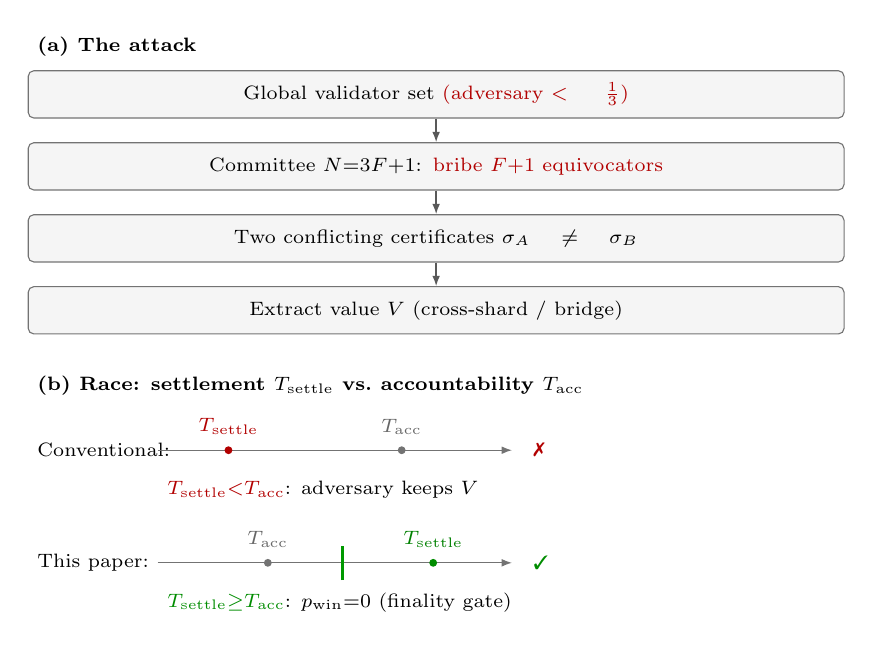
\begin{tikzpicture}[
  font=\scriptsize,
  >={Latex[length=1.3mm]},
  box/.style={rounded corners=2pt, draw=black!55, fill=black!4, align=center,
              inner sep=2.5pt, text width=0.84\columnwidth, minimum height=6mm},
  flow/.style={->, line width=.5pt, black!65},
]
% ---------- (a) the attack (vertical pipeline) ----------
\node[box] (n1) {Global validator set \textcolor{red!70!black}{(adversary $<\tfrac13$)}};
\node[box, below=3mm of n1] (n2) {Committee $N{=}3F{+}1$: \textcolor{red!70!black}{bribe $F{+}1$ equivocators}};
\node[box, below=3mm of n2] (n3) {Two conflicting certificates $\sigma_A\!\neq\!\sigma_B$};
\node[box, below=3mm of n3] (n4) {Extract value $V$ (cross-shard / bridge)};
\draw[flow] (n1)--(n2); \draw[flow] (n2)--(n3); \draw[flow] (n3)--(n4);
\node[anchor=west, font=\scriptsize\bfseries] at ([yshift=3mm]n1.north west) {(a)~The attack};

% ---------- (b) conventional vs.\ ours: the accountability race ----------
\begin{scope}[shift={($(n4.south west)+(0,-0.65)$)}]
  \node[anchor=west, font=\scriptsize\bfseries] at (0,0)
     {(b)~Race: settlement $\Tsettle$ vs.\ accountability $\Tacc$};
  % conventional (ungated): settlement first -> attack pays
  \node[anchor=west] at (0,-0.82) {Conventional:};
  \draw[->, black!55] (1.65,-0.82)--(6.15,-0.82);
  \filldraw[red!70!black] (2.55,-0.82) circle (1.2pt) node[above=2pt, red!70!black] {$\Tsettle$};
  \filldraw[black!55]     (4.75,-0.82) circle (1.2pt) node[above=2pt, black!60] {$\Tacc$};
  \node[anchor=west] at (6.3,-0.82) {\textcolor{red!70!black}{\ding{55}}};
  \node[anchor=west] at (1.65,-1.32) {\textcolor{red!70!black}{$\Tsettle{<}\Tacc$}: adversary keeps $V$};
  % this paper (finality-gated): accountability first -> attack fails
  \node[anchor=west] at (0,-2.25) {This paper:};
  \draw[->, black!55] (1.65,-2.25)--(6.15,-2.25);
  \filldraw[black!55] (3.05,-2.25) circle (1.2pt) node[above=2pt, black!60] {$\Tacc$};
  \draw[green!60!black, line width=.9pt] (4.0,-2.47)--(4.0,-2.03);
  \filldraw[green!55!black] (5.15,-2.25) circle (1.2pt) node[above=2pt, green!50!black] {$\Tsettle$};
  \node[anchor=west] at (6.3,-2.25) {\textcolor{green!55!black}{\ding{51}}};
  \node[anchor=west] at (1.65,-2.75) {\textcolor{green!55!black}{$\Tsettle{\ge}\Tacc$}: $\pwin{=}0$ (finality gate)};
\end{scope}
\end{tikzpicture}
\caption{Overview. \textbf{(a)}~An adversary below the global $\tfrac13$ threshold bribes the $F{+}1$
validators quorum intersection makes \emph{necessary} in one $N{=}3F{+}1$ committee, forging two
conflicting certificates and moving value $V$ across the shard/bridge boundary. \textbf{(b)}~The attack
pays only if value settles before accountability: conventional ungated settlement gives
$\Tsettle{<}\Tacc$ (adversary keeps $V$), whereas gating cross-shard acceptance on finality forces
$\Tsettle{\ge}\Tacc$ and $\pwin{=}0$ (Proposition~\ref{prop:immunity}).}
\label{fig:overview}
\end{figure}

This per-committee argument hides a well-known tension. Because voting power is split, the
\emph{absolute} number of validators an adversary must control to violate safety in one shard is
far smaller than the number required to attack a monolithic chain---a single corrupt committee
``can compromise all the transactions that touch'' it, and detection and recovery remain open
problems~\cite{bano2019sok}. In parallel, a maturing literature shows that validator faults need
not be obtained by intrusion at all: they can be \emph{bought}. Smart contracts can bribe miners
and validators trustlessly~\cite{mccorry2018smart,winzer2019temporary,tran2023crosschain},
game-theoretic analyses price bribery against proof-of-stake \emph{safety}~\cite{karakostas2024bribing},
and recent work implements and evaluates trustless contracts that buy votes, induce validator
exits, and auction randomness-beacon manipulation~\cite{sookitoth2025bribers,kelkar2025omerta,austgen2025liquefaction}.

\paragraph{The composition is not, by itself, an attack.}
Taken together these two strands appear to compose into a devastating attack: pay $F+1$
validators in a small committee to equivocate, and break shard safety for the price of a handful
of bribes. Yet the composition is \emph{not} obviously an attack with consequence. Accountable
BFT consensus turns equivocation into a transferable cryptographic proof and slashes the offending
stake~\cite{buterin2017casper,buchman2018tendermint}. If the adversary forges two conflicting
certificates but the system slashes the bribed validators and reverts the bad branch before any
value moves, the adversary has merely burned the validators' stake and its own bribes for nothing.
The attack's profitability therefore hinges on a question the prior literature does not answer in
the sharded setting: \emph{can the adversary realize value before accountability catches up?}

\paragraph{The accountability race.}
This paper studies that question directly. Our central object is the \emph{accountability race}
(Figure~\ref{fig:overview}) between the time to convert a fraudulently finalized state into irreversible
value---$\Tsettle$, dominated by cross-shard receipt processing and bridge withdrawal beyond
clawback---and the time for the protocol to observe the conflicting certificates, propagate the
equivocation proof, slash, and revert---$\Tacc$. We argue that this race, not the raw cost of
corruption, is what determines whether sub-threshold committee bribery is a real threat to a
given sharded design, and we give the conditions under which it is. Sharding changes the
\emph{economics} of BFT safety: an adversary can buy a \emph{local} shard safety violation after
committee assignment, instead of controlling a large network-wide Byzantine fraction---but the
violation pays only under precise timing and economic conditions, which we make explicit and
checkable.

\paragraph{Two clarifications we treat as load-bearing.}
First, ``sub-threshold'' means below the \emph{network-wide} corruption threshold, \emph{not}
below a committee's local BFT safety threshold: the adversary is globally small but locally
decisive (\S\ref{sec:threat}). Second, the $F+1$ equivocators are \emph{necessary} but not
\emph{sufficient}. By quorum intersection two conflicting $2F{+}1$ certificates must overlap in at
least $F{+}1$ equivocators (Lemma~\ref{lem:intersection}); but each certificate still needs $F$
honest signatures, so the attack also requires honest validators to be \emph{split} across the
two branches---through leader equivocation, message delay, transient asynchrony, network
partition, or protocol-specific scheduling. We fold the probability that a usable split
materializes into a success probability $\psucc$ and never claim that buying $F+1$ equivocations
alone forces a safety break.

\paragraph{Contributions.}
\begin{itemize}
  \item \textbf{A threat model for sub-threshold committee bribery} (\S\ref{sec:threat}) that
  makes precise the sense in which an adversary is globally sub-threshold yet locally decisive,
  and separates the \emph{necessary} purchase of $F+1$ equivocations from the \emph{sufficient}
  honest-split condition captured by $\psucc$.
  \item \textbf{A bribe-cost model} (\S\ref{sec:cost}) in which the equilibrium price of
  equivocation is $b_i \gtrsim q\,(s_i + R_i)$, where $q$ is the probability the fraud proof is
  enforced before the validator's stake becomes unslashable. This connects the cost of corruption
  to accountability latency rather than treating the Byzantine fraction as exogenous.
  \item \textbf{An accountability-race model} (\S\ref{sec:race}) factoring attacker profit into a
  \emph{window} gate $\Tsettle<\Tacc$ and an \emph{economic} gate $V > B + \Cop$, with $\Tacc$ a
  master variable that couples them, and an \emph{immunity-by-construction} result
  (Proposition~\ref{prop:immunity}): finality-gating cross-shard acceptance forces $\pwin=0$.
  \item \textbf{A reconfiguration analysis} (\S\ref{sec:reconf}) that extends the model to
  epoch-boundary state and receipt handoff. We prove a reconfiguration-safe-handoff theorem
  (Proposition~\ref{prop:reconf-safe}) and a residual-vulnerability theorem
  (Proposition~\ref{prop:reconf-residual}), give a taxonomy of six handoff designs, and four
  explicit counterexamples that bound when the attack does \emph{not} apply.
  \item \textbf{A reproducible artifact with a measured testbed and a real-systems case study}
  (\S\ref{sec:impl}--\S\ref{sec:eval}): a seeded simulator, a local proof-of-concept that produces
  genuine equivocation evidence and drives a model \textsc{PayToEquivocate} escrow, and a
  discrete-event BFT testbed with real Ed25519 signatures in which $\Tacc$ and $\Tsettle$ are
  \emph{measured} from a running protocol---independently reproducing the model's $\rho\approx1$
  threshold (the harness also reproduces the closed-form success probability to within Monte-Carlo
  error, max.\ deviation $\ArtifactMaxValErr$). A case study on six deployed systems' documented
  parameters shows that fast evidence ($q\to1$) and finality-gating place them in the safe regime,
  concentrating residual risk in fast-exit, ungated-settlement designs. Every figure and table is
  regenerated from one configuration file.
\end{itemize}

\paragraph{Positioning.}
We do not claim to invent bribery, smart-contract bribery, the observation that small committees
are cheap to corrupt, or cross-shard/bridge value extraction; all are prior art surveyed in
\S\ref{sec:related}. Prior work studies validator bribery, smart-contract bribery, adaptive shard
corruption, and cross-shard attacks \emph{mostly separately}. Our contribution is their
\emph{composition}: post-assignment conditional bribery of a committee-local quorum-intersection
set, \emph{priced by accountability latency}, with profit determined by whether cross-shard or
bridge settlement outruns slashing---together with explicit viability and immunity conditions and
the reconfiguration extension.

\section{Motivation and Problem Statement}
\label{sec:motivation}

\paragraph{What ``sub-threshold'' means.}
Throughout, \emph{sub-threshold} refers to the \emph{network-wide} corruption threshold, not a
committee's local one. A monolithic accountable BFT chain of $n$ validators tolerates up to a
$1/3$ adversarial fraction globally. Our adversary stays comfortably below that global bound, yet
buys enough faults to exceed the local threshold of a \emph{single} committee. The adversary is
thus globally sub-threshold but locally decisive. This is precisely the regime sharding creates
and monolithic analyses miss.

\paragraph{Why the cost of corruption collapses under sharding.}
Consider a network of $n$ validators partitioned into $m$ committees of size $N=n/m$. Attacking a
monolithic chain requires corrupting $\Theta(n)$ validators; attacking one shard requires
corrupting only $F+1 = \lfloor (N-1)/3\rfloor + 1$ validators. For the small committees used in
practice---RapidChain reports committee sizes on the order of a few tens of
nodes~\cite{zamani2018rapidchain}---the per-shard threshold is a handful of validators even when
$n$ is in the thousands. Random assignment and periodic reconfiguration raise the cost of
\emph{targeting} a specific committee, but they do not change the fact that, conditioned on
revealed membership, the local safety margin is small.

\paragraph{Why value is large.}
A shard's finalized state is acted upon as though it were permanent. Cross-shard transaction
protocols move assets between shards on the strength of finalized receipts, and bridges move
assets between chains the same way~\cite{zamyatin2021sok,lee2022sokbridge}. Extractable value $V$
is therefore bounded not by a single shard's local balances but by the liquidity reachable through
its cross-shard and bridge interfaces. The same plumbing that makes sharding useful makes a
single compromised shard valuable to attack.

\paragraph{Why timing is the crux.}
Accountable BFT does not prevent equivocation; it punishes it after the fact. The protective value
of slashing is therefore a function of \emph{latency}: how long after the conflicting certificates
appear can a transfer predicated on the bad branch still be reversed? Cross-shard pipelines are
frequently asynchronous: the source shard finalizes first, emits a receipt, and the destination
shard processes it later, paying gas on the destination side~\cite{harmony2019whitepaper}. If the
destination effect (and any subsequent withdrawal) clears before the source-side equivocation is
proven and the branch reverted, the adversary keeps the proceeds while the bribed validators bear
the slashing. This is the accountability race. Committee reconfiguration does not eliminate this
race; as we show in \S\ref{sec:reconf}, it \emph{relocates} it to the question of whether
old-epoch certified artifacts execute before old-epoch equivocation evidence is enforced.

\paragraph{Problem statement.}
Given a sharded BFT protocol with committee size $N$, a slashing/eviction mechanism with
accountability latency $\Tacc$, and a cross-shard settlement latency $\Tsettle$, we ask:
(i) under what conditions does there exist a window $\Tsettle < \Tacc$ in which fraudulently
finalized state can be converted to irreversible value; (ii) what is the minimum total bribe $B$
required to forge the necessary conflicting certificate; (iii) for which configurations is the
adversary's expected profit positive; and (iv) how does committee reconfiguration at the epoch
boundary change the answer? We seek conditions that are \emph{checkable} against a concrete
design, so that the same analysis serves both as an attack and as a design rule.

\section{Background and Related Work}
\label{sec:related}
\label{sec:background}

\paragraph{Sharded BFT and quorum intersection.}
We assume the now-standard committee-based design~\cite{luu2016elastico,kokoris2018omniledger,zamani2018rapidchain}
in which each shard runs a quorum-based BFT protocol~\cite{castro1999pbft,yin2019hotstuff,buchman2018tendermint}.
The safety of a single shard rests on quorum intersection (Lemma~\ref{lem:intersection}). Cross-shard
atomicity is typically achieved with a two-phase-commit-style protocol coordinated either by the
client or by the shards~\cite{kokoris2018omniledger}; both variants are known to be fragile, as we
discuss below.

\paragraph{Single-shard compromise and adaptive corruption.}
That a committee exceeding its Byzantine threshold compromises all transactions touching it is
identified as an outstanding problem in the canonical systematization~\cite{bano2019sok}. A long
line of sharding work treats the Byzantine fraction as \emph{exogenous} and asks how to make a
captured committee less likely---large committees and unbiasable assignment~\cite{luu2016elastico},
periodic reconfiguration and bounded-adversary epoch models~\cite{zamani2018rapidchain}---or how to
detect capture after the fact. We instead ask what it \emph{costs} to produce the captured committee
once membership is revealed, and what the captor can then extract before accountability resolves.

\paragraph{Adaptive corruption and corrupted-shard tolerance.}
Closest in setting are adaptive-corruption analyses of sharding. \cite{avarikioti2019divide}
formalizes when a sharded ledger stays consistent and scalable against epoch-adaptive versus fully
adaptive adversaries (requiring succinct state-update proofs at epoch boundaries), and
\cite{rana2022free2shard} defends a globally sub-threshold but locally concentrated adaptive adversary
by letting honest nodes re-allocate across shards; \cite{david2022gearbox} minimizes committee size by
separating safety from liveness, which only \emph{amplifies} the leverage of our attack, since smaller
committees are cheaper to bribe. Most directly, the concurrent Camael design~\cite{liu2025camael}
formalizes exactly our structural premise---a single shard exceeding its local BFT threshold (up to
$2/3$ corrupt) while global stake stays below $1/3$---and builds a \emph{defense} that detects
concealed safety violations via snapshots, convicts offenders, and reconfigures the shard. These works
treat the captured committee as a \emph{corruption}-budget event and target consistency, liveness, or
remediation; we treat it as an \emph{economic procurement} event and ask what the captor extracts
before accountability resolves. Tellingly, Camael's snapshot-and-conviction pipeline is itself an
instance of the accountability latency $\Tacc$ our race turns on.

\paragraph{Bribery and crypto-economic security.}
The economic study of buying consensus predates trustless contracts: \cite{bonneau2016rent} showed a
\emph{rented} majority has no long-term stake to protect and is cheap to mobilize, and the
$P{+}\epsilon$ argument~\cite{buterin2015pepsilon} showed a credible conditional payment can make the
adversary's preferred action dominant at near-zero realized cost. Bribing consensus participants via
smart contracts originates with~\cite{mccorry2018smart};
\cite{winzer2019temporary} studies temporary censorship by rational miners (with bribes that are
\emph{not} trustless, as the bribee must trust the briber). \cite{tran2023crosschain} proposes
cross-chain bribery contracts that bribe rational miners in a target network at low cost.
\cite{judmayer2021sok,judmayer2021paytowin} systematize these \emph{algorithmic
incentive-manipulation} attacks and demonstrate cheap, crowdfundable, cross-chain bribery funding a
double-spend on a target chain, and out-of-band collusion contracts~\cite{zhang2023outofband} make
defection the strict equilibrium for a sub-threshold rational coalition, even sketching evasion of
slashing by censoring the proof; that proposer--user side contracts are a fundamental incentive limit
is established by the impossibility of side-contract-proof transaction-fee
mechanisms~\cite{roughgarden2021tfm,chung2023foundations}.
\cite{karakostas2024bribing} gives a game-theoretic treatment of bribery aimed at PoS \emph{safety},
distinguishing \emph{guided} bribes (paid for prescribed behavior) from \emph{effective} bribes
(paid conditional on attack success), and shows that counterincentives---specifically slashing and
dilution---characterize when the attack becomes unprofitable. Most recently,
\cite{sookitoth2025bribers} implements and evaluates three trustless bribery mechanisms on a deployed
PoS system---buying votes to fork, inducing validator exits, and auctioning randomness-beacon
(RANDAO) manipulation---and explicitly debunks the belief that crypto-economic security equals the
total staked value. Modern variants coerce attesters through credible
commitments~\cite{sarenche2024commitment} or buy block delay for MEV without triggering slashing at
all~\cite{yang2024bride}, while \cite{newman2023decentralization} shows the equilibrium per-validator
bribe can fall well below naive expected-loss bounds via low pivotality. Related work studies smart
collusion and whistleblowing as a counterforce to
such contracts~\cite{kelkar2025omerta}, the private liquefaction of staked assets to enable
vote-buying~\cite{austgen2025liquefaction}, and grinding/manipulation of blockchain randomness
beacons~\cite{gazi2025grinding}. These works establish that buying equivocation is feasible,
trustless, and far cheaper than the total-stake figure suggests. They do \emph{not} model the
small-committee quorum structure, the cross-shard realization of the resulting violation, or the way
accountability latency \emph{prices} the bribe.

\paragraph{Economic limits, slashable safety, and accountability latency.}
A separate line bounds attacks economically rather than by a Byzantine fraction. Budish's
flow-versus-stock argument~\cite{budish2018economic} and its permissionless-consensus
generalization~\cite{budish2024economic} establish that an attack is deterred only when its cost
exceeds its profit and---decisively for us---that under partial synchrony above the $1/3$ threshold
targeted punishment \emph{cannot} be enforced before the violator liquidates, an intrinsic
latency-bounded limit on accountability. STAKESURE makes the cost-of-corruption versus
profit-from-corruption gate explicit and caps attacker profit by gating off-chain and bridge value
release on a reversion window~\cite{deb2024stakesure}; CoBRA bounds finalizable value below the
slashable stake so a rational validator's gain cannot exceed its bond~\cite{avarikioti2025cobra}; and
Bitcoin-enhanced PoS makes the unbonding delay the operative security variable, racing slashing
against withdrawal and gating safety on external finality~\cite{tas2023bitcoin}. These results rest on
an accountability substrate we also assume: identifiability of culprits after a
fork~\cite{civit2021polygraph}, per-protocol forensic support fixing how many of the necessary
equivocators are provably catchable~\cite{sheng2021forensics}, the accountable-finalized prefix
underlying finality-gating~\cite{neu2022accountability}, and the detection-and-recovery machinery
whose latency we abstract as $\Tacc$~\cite{gong2025recover}. All study a monolithic, single-chain, or
restaking~\cite{durvasula2025restaking} setting in which the adversary owns stake or value is
throttled, and most assume slashing is effectively immediate. We instead study a globally
\emph{sub-threshold} adversary who, after committee assignment, \emph{buys} the $F{+}1$ equivocators
one $N{=}3F{+}1$ committee makes necessary, prices that bribe by the probability $q$ that the proof is
enforced before stake becomes unslashable, and realizes value across the shard/bridge boundary in
$\Tsettle$ before $\Tacc$; our finality-gating immunity (Proposition~\ref{prop:immunity}) specializes
the accountable-finalized-prefix idea to cross-shard acceptance.

\paragraph{Bribing against an accountability window.}
Closest to our race in spirit is the economic-censorship game of~\cite{berger2025censorship}, in which
an attacker bribes block proposers to censor a defender's challenge transactions and \emph{exhaust the
challenge-period time budget}, with the attacker/defender budget ratio deciding who wins; the
analogous failure where winning a fraud proof is itself unprofitable is studied
by~\cite{lee2025hollow}. This is the same move our $\Tsettle<\Tacc$ gate captures---paying to outlast
accountability---but their adversary censors a single defender's transaction in an
L1$\rightarrow$L2 challenge window, whereas ours buys the quorum-intersection equivocators of an
$N{=}3F{+}1$ committee and races \emph{irreversible cross-shard/bridge} settlement against
detection-and-slashing rather than depleting a fixed challenge clock. The dual defensive
primitive---a remote unbonding protocol that guarantees slashing \emph{before} stake is
withdrawn---is exactly the ``slash before unslashable'' condition our $q$
measures~\cite{dong2024remotestaking}, as is the ``correct until withdrawal'' collateral with
committee resets of~\cite{baron2025aegis}.

\paragraph{Cross-shard, cross-chain, and settlement-before-finality value extraction.}
\cite{sonnino2020replay} presents replay attacks on cross-shard consensus that enable double-spends
and even minting \emph{without subverting any node} and even when Byzantine safety holds---a
different vector from ours (protocol-level message replay, not committee corruption), defended by
their Byzcuit protocol, but clear evidence that cross-shard settlement is a realizable value sink. In
the cross-chain setting, extracting value on a destination and then reverting the source---the
canonical bridge double-mint and reorg-double-spend pattern~\cite{zamyatin2021sok,lee2022sokbridge}---is
precisely the timing move our $\Tsettle<\Tacc$ gate formalizes, but there the reversal is an
opportunistic reorg against a bridge that acts before finality~\cite{schwarzschilling2022three}, not a
reversal manufactured \emph{inside} the protocol by a bribed committee. Miner/maximal-extractable-value
research~\cite{daian2020flashboys} further shows that consensus-level manipulation has directly
monetizable value, and empirical and cross-domain studies quantify the magnitude of such extractable
value~\cite{qin2022quantifying,mcmenamin2023sok}; together these motivate treating $V$ as bounded by
reachable liquidity rather than local balances.

\paragraph{Accountable BFT, slashing, and reconfiguration.}
Accountable consensus turns equivocation into a transferable fraud proof and slashes the offending
stake~\cite{buterin2017casper,buchman2018tendermint}; this is the defender we assume, and the reason
the bare composition of ``small committee'' and ``buyable faults'' is not yet an attack. Sharded
systems additionally rotate committees across epochs and hand off shard state and cross-shard
artifacts at the boundary~\cite{zamani2018rapidchain,kokoris2018omniledger}. Prior work studies
reconfiguration as a means of \emph{raising} adversarial cost (a fresh committee each epoch); we
study how the boundary interacts with accountability, and identify exactly when handoff relocates the
race rather than closing it (\S\ref{sec:reconf}).

\paragraph{Positioning.}
Table~\ref{tab:positioning} situates this work against the closest prior art across the ten
capability dimensions that jointly define the attack. The five \emph{load-bearing} axes are
whether the work \emph{prices} the corruption, whether it is \emph{committee-local}, whether it
models \emph{cross-shard settlement}, whether it models the \emph{accountability race} (value
before slashing), and whether it treats \emph{reconfiguration handoff}; we add five finer
capability columns---a \emph{trustless} payment channel, a \emph{safety} (rather than liveness or
censorship) target, a bribe priced by slashing \emph{latency} $q$, an \emph{immunity} condition,
and an \emph{implemented/measured} artifact---so the comparison is granular rather than coarse.
Read by rows, every prior mechanism leaves at least four columns empty; read by the bottom block,
no prior work addresses more than a handful of the dimensions. Only this work spans all of them,
and that intersection---plus the explicit viability and immunity conditions---is the contribution
of this paper.

\begin{table*}[t]
\centering
\caption{Positioning against the closest prior work across the capability dimensions of the attack.
\yes~addresses it, \partialmark~partially/implicitly, \nomark~does not, \namark~not applicable to
that work's setting. Columns: bribe \emph{priced}; \emph{trustless} payment (no briber--bribee
trust); targets \emph{safety} (vs.\ liveness/censorship); \emph{committee-local} sub-threshold
quorum; cross-shard/bridge \emph{value} realization; the \emph{accountability race} (value before
slashing); bribe priced by slashing \emph{latency} $q$; an \emph{immunity}-by-construction
condition; \emph{reconfiguration} handoff; and an \emph{implemented/measured} artifact. This work
is the only row populated across every dimension.}
\label{tab:positioning}
\scriptsize
\renewcommand{\arraystretch}{1.12}
\setlength{\tabcolsep}{4.5pt}
\begin{tabular}{@{}l l *{10}{c}@{}}
\toprule
\textbf{Work} & \textbf{Setting}
 & \rotatebox[origin=l]{90}{Bribe \emph{priced}\,}
 & \rotatebox[origin=l]{90}{Trustless\,}
 & \rotatebox[origin=l]{90}{Targets \emph{safety}\,}
 & \rotatebox[origin=l]{90}{Committee-local\,}
 & \rotatebox[origin=l]{90}{Cross-shard $V$\,}
 & \rotatebox[origin=l]{90}{Accountability race\,}
 & \rotatebox[origin=l]{90}{Latency-priced $q$\,}
 & \rotatebox[origin=l]{90}{Immunity condition\,}
 & \rotatebox[origin=l]{90}{Reconfig.\ handoff\,}
 & \rotatebox[origin=l]{90}{Impl./measured\,} \\
\midrule
\textbf{This work} & sharded
 & \yes & \yes & \yes & \yes & \yes & \yes & \yes & \yes & \yes & \yes \\
\midrule
\multicolumn{12}{@{}l}{\textit{Bribery mechanisms}}\\
Bribing miners~\cite{mccorry2018smart} & monolithic
 & \yes & \yes & \partialmark & \nomark & \nomark & \nomark & \nomark & \nomark & \nomark & \yes \\
Cross-chain bribery~\cite{tran2023crosschain} & cross-chain
 & \yes & \yes & \partialmark & \nomark & \partialmark & \nomark & \nomark & \nomark & \nomark & \partialmark \\
Pay-to-win~\cite{judmayer2021paytowin} & cross-chain
 & \yes & \yes & \partialmark & \nomark & \partialmark & \nomark & \nomark & \nomark & \nomark & \partialmark \\
Out-of-band collusion~\cite{zhang2023outofband} & monolithic
 & \yes & \yes & \nomark & \partialmark & \nomark & \partialmark & \nomark & \nomark & \nomark & \nomark \\
Bribing \& counterincentives~\cite{karakostas2024bribing} & monolithic
 & \yes & \namark & \yes & \nomark & \partialmark & \partialmark & \nomark & \nomark & \nomark & \nomark \\
BriDe Arbitrager~\cite{yang2024bride} & monolithic
 & \yes & \yes & \nomark & \partialmark & \nomark & \nomark & \nomark & \nomark & \nomark & \yes \\
Trustless bribery contracts~\cite{sookitoth2025bribers} & monolithic
 & \yes & \yes & \partialmark & \nomark & \nomark & \nomark & \nomark & \nomark & \nomark & \yes \\
\addlinespace[1pt]
\multicolumn{12}{@{}l}{\textit{Economic limits and slashable safety}}\\
Economic limits~\cite{budish2024economic} & monolithic
 & \namark & \namark & \yes & \nomark & \nomark & \partialmark & \partialmark & \nomark & \nomark & \nomark \\
STAKESURE~\cite{deb2024stakesure} & restaking
 & \partialmark & \namark & \partialmark & \nomark & \partialmark & \partialmark & \nomark & \yes & \nomark & \nomark \\
CoBRA~\cite{avarikioti2025cobra} & monolithic
 & \namark & \namark & \yes & \nomark & \partialmark & \partialmark & \nomark & \yes & \nomark & \partialmark \\
Bitcoin-enhanced PoS~\cite{tas2023bitcoin} & monolithic
 & \namark & \namark & \yes & \nomark & \nomark & \partialmark & \partialmark & \yes & \partialmark & \partialmark \\
Remote staking~\cite{dong2024remotestaking} & restaking
 & \namark & \namark & \yes & \nomark & \partialmark & \yes & \yes & \partialmark & \partialmark & \nomark \\
\addlinespace[1pt]
\multicolumn{12}{@{}l}{\textit{Accountability-window and sharding}}\\
Economic censorship games~\cite{berger2025censorship} & rollup
 & \partialmark & \namark & \nomark & \nomark & \nomark & \yes & \partialmark & \nomark & \nomark & \nomark \\
Corrupted-shard tolerance~\cite{liu2025camael} & sharded
 & \namark & \namark & \yes & \yes & \partialmark & \nomark & \nomark & \nomark & \partialmark & \yes \\
Cross-shard replay~\cite{sonnino2020replay} & sharded
 & \namark & \namark & \yes & \yes & \yes & \nomark & \nomark & \nomark & \nomark & \yes \\
Free2Shard~\cite{rana2022free2shard} & sharded
 & \namark & \namark & \yes & \yes & \nomark & \nomark & \nomark & \nomark & \partialmark & \partialmark \\
\bottomrule
\end{tabular}
\end{table*}

\section{Threat Model}
\label{sec:threat}

\paragraph{Adversary.}
The adversary $\mathcal{A}$ is a profit-maximizing, computationally bounded party that (i) controls a
budget usable for bribes and gas; (ii) can deploy smart contracts on the sharded system or a
connected chain; (iii) can observe the public mempool, certificates, and committee assignments;
and (iv) may, with bounded probability, induce or exploit transient network asynchrony or occupy a
leader role within the target committee (this is the lever that engineers the honest-vote split
underlying $\psucc$). $\mathcal{A}$ \emph{cannot} break cryptographic primitives, cannot corrupt
more than the network-wide Byzantine threshold across \emph{all} shards simultaneously, and does
not control the randomness used for committee assignment (we treat assignment as given for the
target epoch).

\paragraph{Sub-threshold, precisely.}
$\mathcal{A}$ is \emph{sub-threshold} in the network-wide sense: across the whole validator set it
controls strictly fewer than the global $1/3$ safety threshold. Within the single target committee,
however, it procures $F+1$ equivocating validators---at or above that committee's local threshold.
We never assume $\mathcal{A}$ is below the \emph{local} committee threshold; the entire point is that
the global bound is respected while one committee's bound is not.

\paragraph{Targets and goal.}
$\mathcal{A}$ targets a single committee $C$ of size $N=3F+1$ during one epoch. The goal is to cause
$C$ to finalize two conflicting certificates over shard-local state and to convert the resulting
ambiguity into irreversible value $V$ through the cross-shard or bridge interface, with positive net
profit after bribes, slashing-induced effects, and operating costs. Buying $F+1$ equivocators is
\emph{necessary} (Lemma~\ref{lem:intersection}) but not \emph{sufficient}: $\mathcal{A}$ must also
drive a usable honest-vote split, which succeeds with probability $\psucc$ determined by the protocol
and network (\S\ref{sec:floor}).

\paragraph{Defender.}
The defender runs accountable BFT with a slashing mechanism: provable equivocation by a validator
yields a transferable proof; upon enforcement, the validator's bonded stake $s_i$ is slashed and the
offending branch is reverted or quarantined~\cite{buterin2017casper,buchman2018tendermint}.
Validators have a bonding/unbonding period; let $\Tacc$ denote the end-to-end accountability latency
(detection $\rightarrow$ proof propagation $\rightarrow$ enforcement $\rightarrow$ reversion).
Cross-shard receipts settle with latency $\Tsettle$. We treat a \emph{robust} defender as one whose
stake remains globally bonded and slashable across committee rotation for at least the maximum
evidence delay; \S\ref{sec:reconf} analyzes what happens when this property is weakened.

\paragraph{Assumptions.}
\begin{assumption}[Rational validators]\label{ass:rational}
Each validator maximizes expected payoff and accepts a bribe iff it weakly exceeds the expected cost
of the prescribed behavior.
\end{assumption}
\begin{assumption}[Accountable equivocation]\label{ass:accountable}
Equivocation is detectable and attributable: two validly signed conflicting messages from the same
validator constitute a proof that any honest party can verify and submit.
\end{assumption}
\begin{assumption}[Asynchronous settlement]\label{ass:async}
Cross-shard effects are not gated on the source shard's accountability window unless the protocol
explicitly enforces such gating; absent such a gate, $\Tsettle$ and $\Tacc$ are independent.
\end{assumption}

\section{A Model of Priced Equivocation and the Accountability Race}
\label{sec:design}

We now build the model. Table~\ref{tab:notation} summarizes notation, and Table~\ref{tab:results}
previews the formal results, which we prove in this section and \S\ref{sec:reconf}.

\begin{table}[t]
\centering
\caption{Summary of formal results. The single conditional inequality $\Tsettle<\Tacc$ (gate G1)
governs all of them: closing it yields immunity, leaving it open sustains the attack.}
\label{tab:results}
\small
\begin{tabularx}{\linewidth}{@{}l X l@{}}
\toprule
Result & Statement & Where \\
\midrule
Lemma~\ref{lem:intersection} & Two conflicting commit certificates force $\ge F{+}1$ equivocators
(quorum intersection) & \S\ref{sec:floor} \\
Prop.~\ref{prop:immunity} & Finality-gating cross-shard acceptance forces $\pwin{=}0$, hence
$\mathbb{E}[\Pi]\le0$ (immunity by construction) & \S\ref{sec:race} \\
Prop.~\ref{prop:reconf-safe} & A handoff meeting conditions (i)--(iv) keeps $\pwin{=}0$ for old-epoch
certified artifacts after rotation & \S\ref{sec:reconf} \\
Prop.~\ref{prop:reconf-residual} & Ungated carryover makes $\mathbb{E}[\Pi(a)]$ rise toward the
epoch boundary (residual vulnerability) & \S\ref{sec:reconf} \\
Cex.~\ref{cex:persistent}--\ref{cex:rolling} & Four boundaries where the attack fails: persistent
slashability, gated carryover, cross-shard freeze, rolling reconfiguration & \S\ref{sec:reconf} \\
\bottomrule
\end{tabularx}
\end{table}

\begin{table}[t]
\centering
\caption{Notation for the sub-threshold bribery and accountability-race model.}
\label{tab:notation}
\small
\begin{tabularx}{\linewidth}{@{}lX@{}}
\toprule
Symbol & Meaning \\
\midrule
$N=3F+1$ & committee size; $F$ tolerated faults \\
$Q=2F+1$ & commit quorum size \\
$k=F+1$ & equivocators needed for two conflicting certificates \\
$\varphi$ & view-split: fraction of honest votes on one branch \\
$s_i,\,R_i$ & validator $i$'s bonded stake; continuation value \\
$q$ & Pr[fraud proof enforced before stake unslashable] \\
$b_i,\,B$ & bribe to validator $i$; total bribe $\sum_i b_i$ \\
$\Eval$ & value extractable via the conflicting finality \\
$\Tsettle$ & time to irreversibly realize $\Eval$ \\
$\Tacc$ & accountability latency (detect$\rightarrow$slash$\rightarrow$revert) \\
$\pwin$ & $\Pr[\Tsettle < \Tacc]$ \\
$\psucc$ & $\Pr[\text{conflicting finality}\mid k\text{ equivocators}]$ \\
$\Cop$ & operating cost (gas, infrastructure, stake acquisition) \\
$\Pi$ & adversary net profit \\
\bottomrule
\end{tabularx}
\end{table}

\subsection{The Equivocation Floor (Necessary, Not Sufficient)}
\label{sec:floor}

\begin{lemma}[Equivocation floor]\label{lem:intersection}
In a committee of $N=3F+1$ with commit quorum $Q=2F+1$, any two conflicting commit certificates
share at least $F+1$ signers, each of whom must have signed both branches. Hence at least
$k=F+1$ validators must equivocate.
\end{lemma}
\begin{proof}
Two certificates are sets $Q_1,Q_2$ of signers with $|Q_1|=|Q_2|=2F+1$ drawn from $N=3F+1$ validators.
By inclusion--exclusion, $|Q_1\cap Q_2|\ge |Q_1|+|Q_2|-N = 2(2F+1)-(3F+1)=F+1$. A validator in
$Q_1\cap Q_2$ signed both (conflicting) values, i.e.\ equivocated. Thus $|\{\text{equivocators}\}|\ge F+1$.
\end{proof}

Lemma~\ref{lem:intersection} gives a \emph{necessary} condition. It is emphatically \emph{not}
sufficient: each certificate still needs $Q-(F{+}1)=F$ additional signatures from honest validators,
which requires that the honest validators be \emph{split} across the two branches. We make this
quantitative. Suppose the adversary buys $k\ge F+1$ equivocators; the remaining $H=N-k$ honest
validators each commit to one branch, voting for branch $A$ with probability $\varphi$ (the
view-split the adversary engineers via leader equivocation, message delay, or transient asynchrony).
Branch $A$ finalizes iff $k+h_A\ge Q$ and branch $B$ iff $k+(H-h_A)\ge Q$, where $h_A$ is the number
of honest $A$-votes. Both hold iff
\begin{equation}
Q-k \;\le\; h_A \;\le\; N-Q,
\label{eq:band}
\end{equation}
where the upper bound is the branch-$B$ quorum constraint $k+(H-h_A)\ge Q$ with $H=N-k$, giving
$h_A\le H-(Q{-}k)=N-Q$ \emph{independently of} $k$. This is a feasible band of width $k-F$ for
$F{+}1\le k\le Q$ (exactly $1$ when $k=F+1$, the single point $h_A=N-Q=F$): each equivocator bought
beyond the floor adds exactly one feasible split. Modeling $h_A\sim\mathrm{Binomial}(H,\varphi)$,
\begin{equation}
\psucc(N,k,\varphi) \;=\; \Pr\!\big[\,Q-k \le h_A \le N-Q\,\big].
\label{eq:psucc}
\end{equation}
Two consequences matter. First, at the floor $k=F+1$ the band collapses to the single point
$h_A=F$: an adversary with \emph{no} control over views must hit an exact even split, so $\psucc$ is
modest (for $N=31$, $\psucc=\ArtifactPsuccFloor$ at $\varphi=\tfrac12$). Second, each extra purchased
equivocator widens the band, and $\psucc$ is maximized at $\varphi=\tfrac12$. The adversary therefore
trades bribe budget against split-control, and the two routes to a high $\psucc$ price it very
differently. By an \emph{uncontrolled} split, reaching $\psucc\approx0.85$ at $N=31$ needs $k\approx
F{+}6$ (about half the committee), which raises the bribe to ${\approx}1.45\times$ the $F{+}1$ floor
(at $k{=}F{+}5$, ${\approx}1.36\times$, $\psucc\approx0.79$);
by \emph{view/leader control}---the leader-occupation lever the threat model grants only with bounded
probability (\S\ref{sec:threat})---a near-even split is forced at the floor bribe. Consequently the
profitability analyses of \S\ref{sec:eval} that fix $\psucc=0.85$ adopt the view-control regime, and we
bracket every such result against the uncontrolled-split floor $\psucc=\ArtifactPsuccFloor$ rather than
treat $0.85$ as a default. We treat
$\psucc$ as a protocol-and-network property, not a per-validator cost, and validate
Eq.~\eqref{eq:psucc} against a Monte-Carlo BFT harness in \S\ref{sec:eval}.

\subsection{Bribe-Cost Model}
\label{sec:cost}

Under Assumption~\ref{ass:rational}, validator $i$ equivocates iff the bribe covers its expected
loss. Equivocation is maximally accountable (Assumption~\ref{ass:accountable}): if the proof is
enforced before $i$'s stake becomes unslashable, $i$ loses bonded stake $s_i$ and forfeits
continuation value $R_i$. Let $q=\Pr[\text{proof enforced before } i\text{'s stake unslashable}]$.
Then the individual participation constraint is
\begin{equation}
b_i \;\gtrsim\; q\,(s_i + R_i),
\label{eq:bribe-individual}
\end{equation}
and, summing over the $k=F+1$ required equivocators (homogeneous case $s_i=s,\,R_i=R$),
\begin{equation}
B \;=\; \sum_{i=1}^{F+1} b_i \;\approx\; (F+1)\,q\,(s + R).
\label{eq:bribe-total}
\end{equation}
Equation~\eqref{eq:bribe-total} departs from analyses that equate security with total stake: the
adversary pays for $F+1$ validators, not the whole committee, and pays a \emph{fraction} $q$ of each
one's stake-at-risk rather than its face value. Crucially, $q$ is not a constant of the universe. It
is determined by the defender, through (i) the accountability latency $\Tacc$ relative to the
unbonding/withdrawal delay, (ii) the validity and propagation of equivocation evidence, and (iii) the
reliability of enforcement. We make the latency dependence explicit in \S\ref{sec:race} and the
unbonding/rotation dependence in \S\ref{sec:reconf}, where $q$ becomes a function $q(a)$ of attack
time within the epoch.

\subsection{Value Model}
\label{sec:value}

Let $\Eval$ be the value the adversary can extract by acting on the fraudulently finalized branch
before the conflict is resolved. $\Eval$ is upper-bounded by (i) the liquidity reachable through the
target shard's cross-shard and bridge interfaces within $\Tsettle$, and (ii) the state that the
conflicting certificate can fork (e.g.\ the balances whose double-spend the two branches encode). We
treat $\Eval$ as an exogenous deployment parameter and sweep it in \S\ref{sec:eval}.

\subsection{The Accountability Race}
\label{sec:race}

Start the clock when the conflicting certificate exists ($t=0$). Two latencies compete:
\begin{align*}
\Tsettle &= \text{(dest.\ receipt processing)} \\
         &\quad + \text{(withdrawal beyond clawback)},\\
\Tacc    &= \text{(observe both certs)} + \text{(propagate proof)} \\
         &\quad + \text{(enforce slashing)} + \text{(revert/quarantine)}.
\end{align*}
The adversary retains $\Eval$ only if it settles before accountability lands. Define
$\pwin=\Pr[\Tsettle<\Tacc]$. Combining with the success probability $\psucc$ that $k$ equivocators
actually yield conflicting finality, the realized value is $\psucc\,\pwin\,\Eval$ in expectation. This
product treats the honest-split event (probability $\psucc$) and the window-open event (probability
$\pwin$) as \emph{independent}; we adopt this as a modeling assumption and note its sign. Both are
driven by the same lever---induced asynchrony or leader control raises $\psucc$ and, by delaying
certificate observation and proof propagation, also raises $\pwin$ (the $\Tacc$-as-master-variable
coupling below)---so their covariance is plausibly nonnegative, making the factored $\psucc\,\pwin$ a
\emph{lower} bound on $\mathbb{E}[\psucc\pwin]$ and the break-even $\Eval^{*}\sim1/(\psucc\pwin)$ a
conservative \emph{upper} bound. Immunity ($\pwin=0$) is unaffected.

\paragraph{Profitability.}
With \emph{guided} bribes (paid regardless of outcome, per Assumption~\ref{ass:rational} and
\cite{karakostas2024bribing}) and operating cost $\Cop$, expected profit is
\begin{equation}
\mathbb{E}[\Pi] \;=\; \psucc\,\pwin\,\Eval \;-\; B \;-\; \Cop.
\label{eq:profit-guided}
\end{equation}
With \emph{effective} (success-conditional) bribes, the cost moves inside the success event but
validators demand a premium $B_{\mathrm{succ}}>B$ to bear slashing risk on failed attempts, while
failed attempts may still incur $B_{\mathrm{fail}}\ge 0$:
\begin{equation}
\begin{aligned}
\mathbb{E}[\Pi] ={}& \psucc\,(\pwin\,\Eval - B_{\mathrm{succ}})\\
&{} - (1-\psucc)\,B_{\mathrm{fail}} - \Cop.
\end{aligned}
\label{eq:profit-effective}
\end{equation}
The attack is worth attempting iff $\mathbb{E}[\Pi]>0$. In the deterministic-win, full-success limit
($\psucc=\pwin=1$), \eqref{eq:profit-guided} reduces to a clean pair of \emph{independent gates}:
\begin{align}
\mathrm{(G1)}\quad & \Tsettle < \Tacc, \label{eq:g1}\\
\mathrm{(G2)}\quad & \Eval > B + \Cop, \label{eq:g2}\\
& B=(F{+}1)\,q\,(s{+}R). \nonumber
\end{align}
Both gates must hold. (G1) is a property of the protocol's pipeline and accountability machinery;
(G2) is an economic property of stake, liquidity, and $q$.

\paragraph{$\Tacc$ as a master variable.}
The two gates are coupled through $\Tacc$. A larger $\Tacc$ (slower or less reliable accountability)
raises $\pwin$ in (G1) \emph{and} lowers $q$ in (G2)---validators who expect to escape enforcement
before unbonding accept smaller bribes. Thus slow accountability harms the defender twice: it widens
the settlement window \emph{and} cheapens corruption. ``Cheap to corrupt'' and ``easy to cash out''
are two symptoms of one underlying quantity. This observation, rather than any single inequality, is
the conceptual core of the paper, and it is why purely economic defenses (bigger committees, more
stake) are not a substitute for closing the window.

\begin{proposition}[Immunity by construction]\label{prop:immunity}
If the protocol admits cross-shard (and bridge) effects predicated on a source-shard certificate
only after that certificate is past the source shard's accountability window---formally, if it
guarantees $\Tsettle \ge \Tacc$ for every such effect---then $\pwin=0$, and by
\eqref{eq:profit-guided} $\mathbb{E}[\Pi]=-B-\Cop\le 0$ for any $B\ge 0,\ \Cop\ge 0$, strictly
negative whenever $B+\Cop>0$ (any attack that pays a bribe or gas). No rational
adversary (Assumption~\ref{ass:rational}) mounts the attack, independent of committee size $N$ or
stake $s$.
\end{proposition}
\begin{proof}
By hypothesis every value-realizing cross-shard effect occurs at or after $\Tacc$, so
$\Pr[\Tsettle<\Tacc]=0$, i.e.\ $\pwin=0$. Substituting into \eqref{eq:profit-guided} gives
$\mathbb{E}[\Pi]=-(B+\Cop)\le 0$, strictly negative whenever the adversary pays any bribe or gas. Under
Assumption~\ref{ass:rational} the adversary declines a strictly negative-expectation action.
\end{proof}

Proposition~\ref{prop:immunity} is a design rule as much as a theorem: it states the exact condition
a sharded system must enforce to be unconditionally safe against this attack, and explains why
enlarging committees or stake (which affect only (G2)) does not help once (G1) is open.

\subsection{Attack Procedure}
\label{sec:procedure}

Algorithm~\ref{alg:attack} states the end-to-end procedure; Figure~\ref{fig:flow} depicts it. The
trustless payment mechanism is a contract that releases a bribe only upon submission of a valid
equivocation proof by a registered validator, so neither party need trust the other
(cf.~\cite{sookitoth2025bribers}). Appendix~\ref{app:contract} sketches the contract; \S\ref{sec:impl}
reports a runnable local model of the same logic.

\begin{figure}[t]
\centering
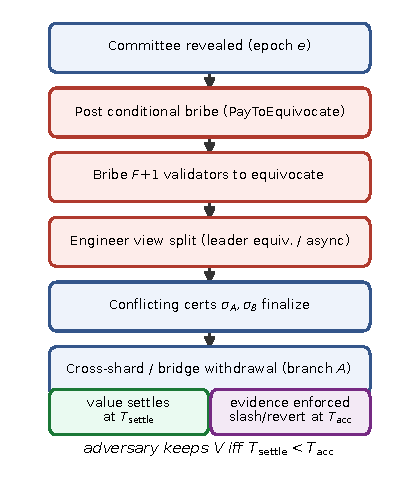
\includegraphics[width=0.86\linewidth]{fig1_attack_flow.pdf}
\caption{Sub-threshold committee bribery and the accountability race. The adversary retains $V$ only
if cross-shard settlement ($\Tsettle$) precedes end-to-end accountability ($\Tacc$).}
\label{fig:flow}
\end{figure}

\begin{algorithm}[t]
\caption{Sub-threshold committee bribery with accountability race}
\label{alg:attack}
\begin{algorithmic}[1]
\State \textbf{Input:} target committee $C$ ($|C|=3F{+}1$), value target $\Eval$, budget
\State Estimate $\Tacc,\Tsettle,q$ for $C$ and its cross-shard interface
\If{$\Tsettle \ge \Tacc$ \textbf{or} $\Eval \le (F{+}1)q(s{+}R)+\Cop$}
  \State \textbf{abort} \Comment{a gate fails; not profitable (cf.\ Prop.~\ref{prop:immunity})}
\EndIf
\State Deploy \textsc{PayToEquivocate} escrow funded with $B \approx (F{+}1)q(s{+}R)$
\State Recruit $k=F{+}1$ validators of $C$ to register and commit to equivocate
\State Engineer/await a usable view (leader equivocation or transient asynchrony) so honest
       validators split across branches $b_A \ne b_B$
\State Drive $C$ to finalize conflicting certificates $\sigma_A$ on $b_A$ and $\sigma_B$ on $b_B$
\State On branch $b_A$, submit the cross-shard receipt that moves/duplicates $\Eval$
\State Withdraw $\Eval$ on the destination beyond clawback \Comment{completes at $\Tsettle$}
\State Bribed validators submit equivocation proofs to \textsc{PayToEquivocate}; bribes released
\State \textbf{Outcome:} if completed before $\Tacc$, adversary retains $\Eval$; bribed validators
       are slashed
\end{algorithmic}
\end{algorithm}


\section{Reconfiguration-Phase Accountability Races}
\label{sec:reconf}

A reviewer's first question about any single-shard, single-epoch attack is: what happens when
validators rotate among shards? Sharded systems reassign committees and hand off shard state and
cross-shard artifacts at epoch boundaries~\cite{zamani2018rapidchain,kokoris2018omniledger}. This
section extends the model to that boundary. Its thesis is deliberately narrow:
\emph{reconfiguration does not eliminate the accountability race; it relocates it.} Whether
relocation helps the attacker or the defender depends entirely on how old-epoch certified artifacts
are handed off, and we give the exact condition (Propositions~\ref{prop:reconf-safe}
and~\ref{prop:reconf-residual}).

\paragraph{Three events that must be distinguished.}
We do \emph{not} claim that validator rotation lets bribed validators escape slashing. Robust
PoS/BFT systems separate three events that a careless analysis conflates:
(1) \emph{shard rotation}---a validator leaves shard $A$ and joins shard $B$;
(2) \emph{validator exit}---a validator stops validating; and
(3) \emph{stake withdrawal}---a validator recovers bonded stake and is no longer slashable.
A validator that merely rotates out of a shard should remain slashable for old-epoch equivocation,
because the evidence---validator identity, shard ID, epoch, height/round, and the two conflicting
signed values---is self-contained and can be enforced by a global staking/beacon layer after
rotation (Counterexample~\ref{cex:persistent}). The attack's reconfiguration angle is therefore
\emph{not} ``rotation defeats slashing''; it is whether a \emph{value-bearing certified artifact}
created by the old committee can execute in the next epoch before old-epoch evidence is enforced.

\paragraph{Variables.}
Let $\tau$ be the epoch length and $a\in[0,\tau]$ the attack time within the epoch, with
$r=\tau-a$ the remaining time before nominal reconfiguration. Let $U$ be the unbonding/withdrawal
delay after validator exit, $\Hreconf(a)$ the extra accountability delay caused by committee handoff,
state transfer, beacon processing, or proof routing across epochs, $\Tstate$ the time for the new
committee to obtain and verify shard state, $\Treceipt$ the time for old-epoch receipts/locks/
withdrawal certificates/outbox messages to become executable in the next epoch, and $\Tevid$ the time
for old-epoch equivocation evidence to become enforceable against globally bonded stake. Finally,
$q(a)=\Pr[\text{evidence enforced before stake unslashable}]$ generalizes the enforcement
probability $q$ of \S\ref{sec:cost} to attack time $a$.

\paragraph{Extended profit model.}
The single-epoch model of \S\ref{sec:design} becomes, as a function of attack time,
\begin{equation}
\mathbb{E}[\Pi(a)] \;=\; \psucc(a)\,\pwin(a)\,\Eval \;-\; B(a) \;-\; \Cop,
\label{eq:profit-a}
\end{equation}
with $B(a)=(F{+}1)\,q(a)\,(s{+}R)$. The window term depends on the handoff design. For
\emph{receipt-carryover} designs, where the old-epoch artifact survives into epoch $e{+}1$ and
executes there,
\begin{equation}
\pwin(a)=\Pr\big[\,\Tsettle^{\mathrm{ce}} < \Tacc + \Hreconf(a)\,\big],
\label{eq:pwin-carry}
\end{equation}
where the cross-epoch settlement time $\Tsettle^{\mathrm{ce}}=\Treceipt+\Tstate+\Twd$ (with $\Twd$
the destination withdrawal) must beat $\Tevid$: the handoff penalty $\Hreconf(a)$ \emph{widens} the
effective accountability deadline, so the artifact need only beat $\Tevid$. For
\emph{hard-cutoff} designs, where the old committee stops at the boundary and no value-bearing
artifact may execute afterward,
\begin{equation}
\pwin(a)=\Pr\big[\,\Tsettle < \min(\Tacc,\,r)\,\big].
\label{eq:pwin-cut}
\end{equation}
As $a\to\tau$ we have $r\to0$, so last-block attacks become \emph{useless} under a hard cutoff unless
the malicious artifact was already certified and settles within the shrinking $r$. The two regimes
pull $\mathbb{E}[\Pi(a)]$ in opposite directions near the boundary; Figure~\ref{fig:reconf-profit}
shows the resulting curves.

\subsection{What Survives Reconfiguration}
\label{sec:survives}

Ordinary mempool transactions are \emph{not} the main risk. A pending transaction can be dropped,
retried, re-gossiped, or carried into the next epoch without ever being consensus-final; nothing
value-bearing has been certified. The dangerous objects are old-epoch \emph{certified} artifacts:
finalized shard headers, state roots, receipt/outbox roots, pending incoming receipts, cross-shard
locks, withdrawal certificates, and bridge-relevant certificates. The attack matters precisely when
an old committee creates a certified value-bearing artifact that remains \emph{executable} after
reconfiguration but before old-epoch equivocation evidence is enforced. We therefore restate the
race in handoff terms:

\begin{quote}
\emph{Reconfiguration does not eliminate the accountability race; it relocates it. Even if the old
committee stops producing blocks, certified receipts, locks, and state roots may survive into the
next epoch. The relevant residual window is not the time left to produce ordinary blocks, but the
time during which old-epoch artifacts remain executable before old-epoch equivocation evidence is
enforced.}
\end{quote}

\subsection{A Taxonomy of Reconfiguration Designs}
\label{sec:taxonomy}

Table~\ref{tab:taxonomy} classifies the handoff designs by what they do at the boundary and the
condition under which each is safe or dangerous. Figure~\ref{fig:reconf-fsm} renders the handoff as a
state machine with the safe (gated) and unsafe (ungated) paths.

\begin{table*}[t]
\centering
\caption{Reconfiguration designs and their effect on the attack. ``Safe'' is the condition under
which $\pwin\to0$ for old-epoch value-bearing artifacts (Proposition~\ref{prop:reconf-safe});
``dangerous'' is the residual-vulnerability condition (Proposition~\ref{prop:reconf-residual}).}
\label{tab:taxonomy}
\small
\begin{tabularx}{\textwidth}{@{}l X X X X@{}}
\toprule
Design & At the epoch boundary & Effect on attack & Safe condition & Dangerous condition \\
\midrule
A. Hard cutoff + mempool carryover & Old committee stops; unincluded txns retried/re-gossiped & Last-block attack weak unless the malicious tx was already certified & Value-bearing artifacts cannot execute after the cutoff & A receipt was certified before the cutoff and settles within $r$ \\
B. Drain phase & Protocol stops accepting new cross-shard txns and finishes pending locks/receipts before rotation & Strong if drained receipts execute before accountability & Pending receipts held through the accountability window & Drained receipts execute immediately at boundary \\
C. Receipt/outbox handoff & Old-epoch receipts/outbox imported in epoch $e{+}1$ & The most important case: artifact survives and executes next epoch & Import is accountability-gated (held until evidence window elapses) & Imported receipts executed immediately on import \\
D. Old/new committee overlap & Old committee signs final checkpoint; new committee signs import checkpoint & Depends on whether the new committee checks for conflicts & New committee rejects/quarantines conflicting old certificates & New committee blindly imports one old root \\
E. Global beacon/control-layer checkpoint & Beacon records shard headers, receipt roots, assignments, slashing evidence & Preserves accountability across rotation & Beacon quarantines old receipt roots until evidence can land & Beacon finalizes old receipt roots before evidence is enforced \\
F. Rolling/asynchronous reconfiguration & Validators rotate gradually; no single last-block cliff & No cutoff, but attacker optimizes $a$ via $q(a),\Tstate,\Tevid$ & Old-epoch artifacts stay gated throughout the roll & Some artifacts execute during the roll before evidence \\
\bottomrule
\end{tabularx}
\end{table*}

\begin{figure}[t]
\centering
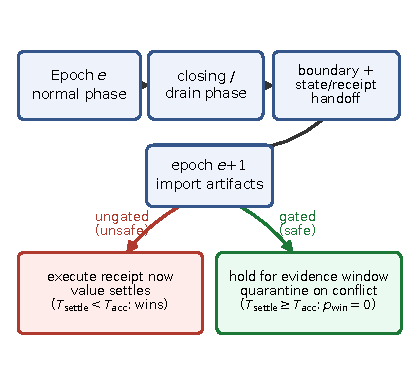
\includegraphics[width=0.96\linewidth]{fig5_reconf_fsm.pdf}
\caption{Epoch-boundary handoff as a state machine. The safe (accountability-gated) path quarantines
old-epoch artifacts until evidence can land ($\pwin=0$); the unsafe (ungated) path executes them
immediately, reopening the race.}
\label{fig:reconf-fsm}
\end{figure}

\subsection{State Handoff Under Committee Rotation}
\label{sec:handoff}

New validators must obtain shard state before they can validate. Mechanisms include a full snapshot
transfer verified against a state root; a checkpoint plus block replay; stateless validation with
witnesses/Merkle proofs; old/new committee checkpoint overlap; a global beacon/control-layer shard
header; and erasure-coded or data-availability-backed state reconstruction. Crucially, the new
committee needs more than account balances. It needs the (1) latest finalized shard header,
(2) state root, (3) receipt/outbox root, (4) pending incoming receipts, (5) pending cross-shard
locks, (6) withdrawal certificates, (7) validator-assignment metadata, (8) old-epoch
equivocation/slashing evidence, and optionally (9) mempool transactions. Of these, mempool state is
\emph{not} consensus-critical---it can be reconstructed or dropped---whereas receipt roots, locks,
finalized headers, and equivocation evidence \emph{are}. A handoff that imports value-bearing roots
(3)--(6) without first importing and checking evidence (8), and without gating execution behind the
source accountability window, is exactly the dangerous case of Table~\ref{tab:taxonomy}.

\subsection{Counterexamples: When the Attack Does Not Apply}
\label{sec:counterexamples}

Precise threat models name their boundaries. The following cases make the reconfiguration angle
reviewer-resistant by stating when it fails.

\begin{counterexample}[Persistent slashability after rotation]\label{cex:persistent}
A validator rotates from shard $A$ to shard $B$, but its stake remains globally bonded. The
equivocation evidence (identity, shard ID, epoch, height/round, conflicting signed values) is
self-contained, so a global slashing contract or beacon layer can slash after rotation. Shard
rotation therefore does \emph{not} imply accountability escape; $q(a)$ stays high and $B(a)$ does not
fall.
\end{counterexample}

\begin{counterexample}[Accountability-gated receipt carryover]\label{cex:gated}
Old-epoch receipts carry into epoch $e{+}1$ but remain \emph{pending} through a challenge/
accountability window. If equivocation evidence appears, the receipt root is quarantined and the
validators slashed. This enforces $\Tsettle\ge\Tacc$ and gives $\pwin=0$ (Figure~\ref{fig:reconf-profit},
flat line): the attack is killed regardless of $a$.
\end{counterexample}

\begin{counterexample}[Cross-shard freeze during reconfiguration]\label{cex:freeze}
The protocol allows local transactions but freezes cross-shard receipt execution during state
handoff. Last-block cross-shard attacks fail because no value-bearing artifact can settle across the
boundary.
\end{counterexample}

\begin{counterexample}[Rolling reconfiguration]\label{cex:rolling}
There is no single point where the old committee disappears, so there is no last-block escape to
exploit. The attack must be modeled continuously; with old-epoch artifacts gated throughout the roll,
$\pwin$ never opens (Figure~\ref{fig:reconf-profit}, rolling curve stays bounded).
\end{counterexample}

These cases do not weaken the paper; they sharpen its threat model.

\subsection{Two Propositions}
\label{sec:reconf-props}

\begin{proposition}[Reconfiguration-safe handoff]\label{prop:reconf-safe}
Suppose a sharded protocol satisfies all of:
\emph{(i)} old-epoch equivocation evidence remains valid and enforceable after committee rotation;
\emph{(ii)} validator stake remains bonded and slashable for at least the maximum evidence delay
$\Tevid$;
\emph{(iii)} old-epoch receipts, locks, and withdrawal certificates are not executable until the
corresponding source-shard accountability window has elapsed; and
\emph{(iv)} the new committee verifies imported state, receipt roots, and pending artifacts against a
canonical checkpoint and rejects/quarantines conflicting old-epoch certificates.
Then committee reconfiguration does not increase the adversary's settlement-before-accountability
probability for old-epoch artifacts; in particular, accountability-gated old-epoch artifacts have
$\pwin=0$.
\end{proposition}
\begin{proof}
See Appendix~\ref{app:proofs}.
\end{proof}

\begin{proposition}[Reconfiguration-residual vulnerability]\label{prop:reconf-residual}
Suppose instead that the protocol allows old-epoch certified receipts, locks, or withdrawal artifacts
to become executable in epoch $e{+}1$ before old-epoch equivocation evidence can be enforced
(violating (iii)), and that reconfiguration either increases accountability latency by $\Hreconf(a)$
with $\Hreconf$ nondecreasing in $a$, or decreases $q(a)$ near the epoch boundary. Then there is a
boundary region $[\tau-\delta,\tau]$ on which $\mathbb{E}[\Pi(a)]$ is increasing in $a$; attacking
near the end of the epoch strictly increases expected adversarial profit relative to a mid-epoch
attack.
\end{proposition}
\begin{proof}
See Appendix~\ref{app:proofs}.
\end{proof}

\begin{figure}[t]
\centering
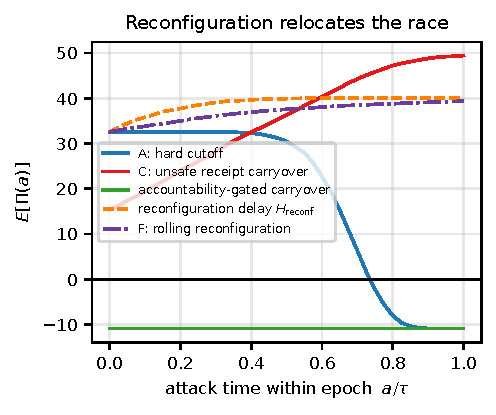
\includegraphics[width=\linewidth]{fig6_reconf_profit.pdf}
\caption{Expected profit $\mathbb{E}[\Pi(a)]$ across the epoch for each handoff design
(\S\ref{sec:eval}, $N=31$, $V=60s$). Hard cutoff (A) collapses as $a\to\tau$ (residual time $r\to0$);
unsafe carryover (C) and reconfiguration-delay designs \emph{rise} toward the boundary
(Proposition~\ref{prop:reconf-residual}); accountability-gated carryover stays flat and negative
($\pwin=0$, Proposition~\ref{prop:reconf-safe}); rolling reconfiguration (F) has no cliff.}
\label{fig:reconf-profit}
\end{figure}

\section{Implementation and Artifact}
\label{sec:impl}

We implement the model as a seeded artifact (\,$\sim$1{,}900 lines of Python over the standard library
plus \texttt{numpy}, with \texttt{cryptography} for Ed25519 and \texttt{matplotlib}/\texttt{pyyaml}). It
has three layers: an \emph{analysis} layer that evaluates the closed-form model and its Monte-Carlo
counterparts; a \emph{proof-of-concept} that runs the attack end-to-end on an abstract committee; and a
\emph{discrete-event testbed} in which the race latencies are \emph{measured outputs} of a running
protocol, not inputs. Two properties are load-bearing for the evaluation. First, the testbed gives each
validator a real Ed25519 keypair, delivers every message after a heavy-tailed per-link latency, and
derives $\Tacc$ and $\Tsettle$ from event timing---so the agreement between testbed and closed form
(\S\ref{sec:eval}, Fig.~\ref{fig:testbed}) is a genuine cross-validation rather than a tautology, and
the equivocation evidence is a real $\ArtifactEvidenceBytes$-byte pair of $\ArtifactSigBytes$-byte
signatures over conflicting values. Second, the driver \emph{self-validates} before producing any
result (\S\ref{sec:eval}): the Monte-Carlo harness must reproduce the closed-form $\psucc$ to tolerance,
a sub-floor purchase ($k<F{+}1$) must yield zero conflicting certificates, and the end-to-end PoC must
emit valid evidence and a paying escrow. The three layers share a single core: one component is the
source of truth for the equations of \S\ref{sec:design}, an \emph{independent} Monte-Carlo estimator
cross-checks $\psucc$, and the testbed derives the race latencies; the reconfiguration analysis, the
real-systems case study, and the read-only live measurement of \S\ref{sec:measured} reuse the same
core rather than re-deriving its quantities. A module-by-module map of the artifact, together with the
reproduction commands and the parameter file, is given in Appendix~\ref{app:repro}
(Table~\ref{tab:artifact}); the live-measurement collectors are read-only over public data.

\section{Experimental Setup}
\label{sec:setup}

\paragraph{Methodology and provenance.}
The evaluation has five layers, each reproducible from \texttt{configs/main.yaml}:
(1) the \emph{closed-form model} of \S\ref{sec:design}--\S\ref{sec:reconf};
(2) \emph{Monte-Carlo simulators} that independently estimate the two probabilistic quantities
($\psucc$ from the BFT quorum harness, $\pwin$ from the accountability-race simulator) and are checked
against the closed form;
(3) a \emph{local proof-of-concept} that runs the end-to-end attack on an abstract BFT committee,
producing real equivocation evidence and a paying escrow;
(4) a \emph{discrete-event testbed} with real Ed25519 signatures in which $\Tacc$ and $\Tsettle$ are
measured from a running protocol and cross-validated against the closed form; and
(5) a \emph{case study} that evaluates the model at the documented parameters of deployed systems. No
quantity in \S\ref{sec:eval} is a hand-chosen placeholder: each is computed by the artifact, and the
figures/tables are regenerated by the commands of \S\ref{sec:impl}. We do not \emph{actively} measure
a live deployed network under attack; that is the stated next step in \S\ref{sec:limitations}, and the
testbed and case study are structured so that each quantity has a live counterpart to instrument.

\paragraph{Live-measurement hook.}
For a concrete deployment, the two load-bearing quantities can be measured without executing an
attack by instrumenting timestamps for: source certificate creation; destination receipt acceptance;
withdrawal or bridge finalization; first observation of conflicting certificates; evidence
propagation to the accountability layer; slashing/quarantine effectiveness; and stake withdrawal or
unbonding completion. These logs give $\Tsettle$ directly, give $\Tacc$ from evidence observation to
effective enforcement, and estimate
$q=\Pr[t_{\mathrm{slash}}<t_{\mathrm{withdraw}}]$ under the deployment's normal evidence and
unbonding rules. The local testbed uses the same timestamp schema, which is why its outputs are a
drop-in rehearsal for the production measurement.

\paragraph{Parameters and sweeps.}
Table~\ref{tab:params} lists parameters and swept ranges. We study committee sizes from small
practical committees to large ones; enforcement probability $q$ from ``accountability rarely lands in
time'' to ``near-certain''; and the latency ratio $\rho=\Tacc/\Tsettle$ across the critical point
$\rho=1$. We treat $\psucc$ as the adversary's split-control reliability; we fix it at the strong-split
value $0.85$---the \emph{view-control} regime, or $k\approx F{+}6$ at ${\approx}1.45\times$ the floor
bribe by an uncontrolled split (\S\ref{sec:floor})---for the window analyses, and sweep it
$\psucc\in[\ArtifactPsuccFloor,1]$ for sensitivity, reporting alongside the random-split \emph{floor}
of Eq.~\eqref{eq:psucc}.

\begin{table}[t]
\centering
\caption{Simulation parameters and swept ranges (from \texttt{configs/main.yaml}).}
\label{tab:params}
\small
\begin{tabularx}{\linewidth}{@{}llX@{}}
\toprule
Parameter & Symbol & Range (swept) \\
\midrule
Committee size & $N=3F{+}1$ & $\{4,7,\ldots,400\}$ (8 sizes) \\
Equivocators & $k=F{+}1$ & derived from $N$ \\
View-split & $\varphi$ & $[0.02,\,0.98]$ \\
Stake at risk & $s$ & normalized to $1$ \\
Continuation value & $R$ & $\{0,\,0.5\,s,\,s\}$ \\
Enforcement prob. & $q$ & $[0.05,\,1.0]$ \\
Latency ratio & $\rho=\Tacc/\Tsettle$ & $[0.25,\,4]$ \\
Settle-time CV & $\mathrm{CV}_{\Tsettle}$ & $\{0.1,0.3\}$ \\
Extractable value & $\Eval$ & $[0,\,200]\cdot s$ \\
Split-control & $\psucc$ & floor $\ArtifactPsuccFloor$ to $1$; $0.85$ = view-control \\
Epoch length & $\tau$ & $1$ (normalized) \\
Unbonding delay & $U$ & $0.15\,\tau$ \\
Cross-epoch latencies & $\Treceipt,\Tstate$ & $0.10,\,0.08$ \\
Handoff penalty (max) & $\Hreconf$ & $0.40$ \\
Monte-Carlo trials & --- & up to $6{\times}10^4$ \\
\bottomrule
\end{tabularx}
\end{table}

\paragraph{Metrics.}
We report (i) $\psucc$ vs.\ $\varphi$ for $k\in\{F{+}1,F{+}2,F{+}3\}$ with a Monte-Carlo overlay;
(ii) the window-open probability $\pwin$ vs.\ $\rho$ and settle-time variance; (iii) the minimum bribe
$B$ vs.\ $N$ and $q$; (iv) the break-even value $\Eval^{*}=B+\Cop$; (v) expected profit
$\mathbb{E}[\Pi]$ over the $(\rho,\Eval)$ and $(q,\Eval)$ planes; (vi) $\mathbb{E}[\Pi(a)]$ across the
epoch for each handoff design; and (vii) the effect of each defense on $\mathbb{E}[\Pi]$.

\paragraph{Baselines.}
As an immunity baseline we include the finality-gated configuration of
Proposition~\ref{prop:immunity} ($\pwin\equiv0$), against which any profitable region must vanish, and
the accountability-gated carryover of Proposition~\ref{prop:reconf-safe} for the reconfiguration
sweep.

\section{Evaluation}
\label{sec:eval}

We organize the evaluation around seven research questions, preceded by a validation step that
establishes the simulator and the proof-of-concept are sound. RQ1--RQ5 exercise the model; RQ6
cross-validates it against a discrete-event testbed with real signatures; RQ7 applies it to the
documented parameters of deployed systems. All numbers are produced by the artifact
(\S\ref{sec:impl}); figure and table references are to artifact output.

\paragraph{Validation and proof-of-concept (RQ0).}
The Monte-Carlo BFT harness reproduces the closed-form $\psucc$ of Eq.~\eqref{eq:psucc} across all
tested $(N,\varphi)$ with maximum absolute deviation $\ArtifactMaxValErr$ (tolerance $0.02$),
validating both the harness and the closed form. A sub-floor purchase ($k<F{+}1$) yields a conflicting
certificate in \emph{zero} of every trial, confirming Lemma~\ref{lem:intersection} empirically. The
end-to-end PoC, on a committee of $N=\ArtifactPoCN$ ($F=10$, floor $k=\ArtifactPoCk$), drives both
branches to the quorum $Q=21$ under an engineered split, emits $\ArtifactPoCEvidence$ valid
equivocation proofs, and the \textsc{PayToEquivocate} escrow pays exactly those $\ArtifactPoCBribes$
and rejects a forged (non-conflicting) proof. The attack is therefore realizable end-to-end in the
local model, not merely asserted.

\paragraph{The floor is necessary, not sufficient.}
Figure~\ref{fig:psucc} plots $\psucc$ against the view-split $\varphi$ for $k\in\{F{+}1,F{+}2,F{+}3\}$,
with the Monte-Carlo overlay matching the closed form. At the floor $k=F{+}1$, success requires an
exact even split, so $\psucc$ peaks at only $\ArtifactPsuccFloor$ at $\varphi=\tfrac12$ and falls off
sharply for asymmetric splits; each extra purchased equivocator widens the feasible band
(Eq.~\eqref{eq:band}) and raises $\psucc$. This quantifies the central caveat: buying the $F{+}1$
floor is necessary but, without engineering a balanced honest split, far from sufficient.

\begin{figure}[t]
\centering
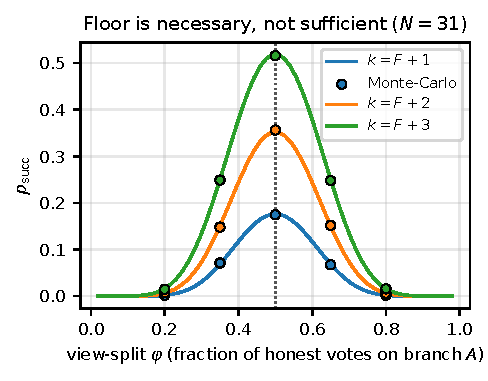
\includegraphics[width=\linewidth]{fig_psucc.pdf}
\caption{$\psucc$ vs.\ view-split $\varphi$ for the floor and two larger purchases ($N=31$). Markers:
Monte-Carlo harness; lines: closed form (Eq.~\eqref{eq:psucc}).}
\label{fig:psucc}
\end{figure}

\paragraph{RQ1: When does the settlement window open?}
The window is nearly a step function---there is almost no middle ground between closed and open. The
window-open probability $\pwin$ crosses $0.5$ within $1\%$ of $\rho=\Tacc/\Tsettle=1$ and saturates
toward $1$ for $\rho\gg1$ (Figure~\ref{fig:pwin}), with higher settle-time variance softening the
transition, exactly as the model predicts. The finality-gated baseline (Proposition~\ref{prop:immunity})
is identically zero for all $\rho$---the flat line at the bottom---so closing the window is not a matter
of degree but of construction.

\begin{figure}[t]
\centering
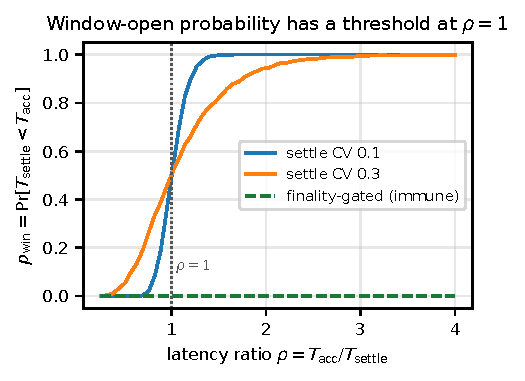
\includegraphics[width=\linewidth]{fig_pwin.pdf}
\caption{RQ1. Window-open probability $\pwin$ vs.\ latency ratio $\rho$, for two settle-time
coefficients of variation, plus the finality-gated immunity baseline ($\pwin\equiv0$).}
\label{fig:pwin}
\end{figure}

\paragraph{RQ2: How does the bribe cost scale?}
The bribe is strikingly small relative to the committee: at $N=31,\,q=0.5,\,R=0.5s$ the minimum total
bribe is just $8.25s$---the adversary pays $F{+}1{=}11$ validators a \emph{fraction} $q$ of their
stake-at-risk, not the whole committee's stake. Figure~\ref{fig:cost} plots $B=(F{+}1)q(s{+}R)$ against
committee size $N$ for several $q$: cost grows only \emph{linearly} in $N$ (through $F{+}1$) and
linearly in $q$. The policy reading is that raising $N$ increases the (G2) cost only linearly,
whereas closing (G1) removes the threat outright---consistent with Proposition~\ref{prop:immunity} and
quantified in RQ5.

\begin{figure}[t]
\centering
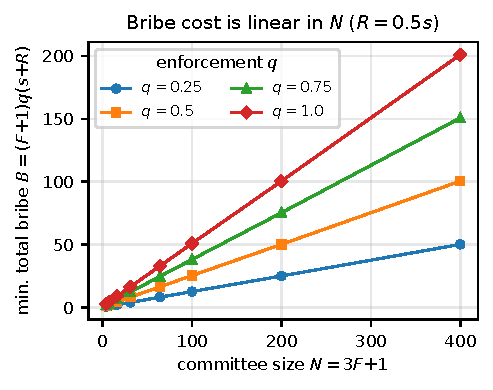
\includegraphics[width=\linewidth]{fig4_cost.pdf}
\caption{RQ2. Minimum total bribe $B$ vs.\ committee size $N$ for $q\in\{0.25,0.5,0.75,1.0\}$,
$R=0.5s$.}
\label{fig:cost}
\end{figure}

\paragraph{RQ3: When is the attack profitable?}
Profit lives in a single quadrant: both gates must hold at once. Figure~\ref{fig:phase} shows
$\mathbb{E}[\Pi]$ over the $(\rho,\Eval)$ plane is positive only in the upper-right region where
$\rho>1$ \emph{and} $\Eval>\Eval^{*}$; the finality-gated baseline collapses the entire plane to
non-positive profit. Table~\ref{tab:breakeven} reports the break-even value
$\Eval^{*}=(F{+}1)q(s{+}R)+\Cop$ across $N$ and $q$. Figure~\ref{fig:profitqV}
slices the profitable region over $(q,\Eval)$ at a window-open $\rho$, showing the linear shift of the
break-even frontier with $q$. Sensitivity to the adversary's split-control reliability is direct: the
break-even value scales as $1/(\psucc\pwin)$, so a weak adversary ($\psucc=0.2$) needs roughly
$4{\times}$ the value of a strong one ($\psucc=0.85$) to clear (G2). We do not treat $\psucc=0.85$ as a
default: it is the view-control regime; an uncontrolled split caps $\psucc$ at $\ArtifactPsuccFloor$ at
the $F{+}1$ floor, and reaching $0.85$ by purchase alone costs $k\approx F{+}6$ at a $1.45\times$ bribe
(\S\ref{sec:floor}). The phase diagram (Fig.~\ref{fig:phase}) is thus the strong-adversary upper edge of
a band whose lower edge is the floor.

\begin{table}[t]
\centering
\caption{RQ3. Break-even extractable value $\Eval^{*}=(F{+}1)q(s{+}R)+\Cop$ (units of $s$; $R=0.5s$,
$\Cop=1$).}
\label{tab:breakeven}
\small
% AUTO-GENERATED by artifact/make_tables.py -- do not edit by hand.
\begin{tabular}{@{}lcccc@{}}
\toprule
$N$ ($k{=}F{+}1$) & $q{=}0.25$ & $q{=}0.5$ & $q{=}0.75$ & $q{=}1.0$ \\
\midrule
$4$ ($2$) & 1.75 & 2.50 & 3.25 & 4.00 \\
$7$ ($3$) & 2.12 & 3.25 & 4.38 & 5.50 \\
$16$ ($6$) & 3.25 & 5.50 & 7.75 & 10.00 \\
$31$ ($11$) & 5.12 & 9.25 & 13.38 & 17.50 \\
$64$ ($22$) & 9.25 & 17.50 & 25.75 & 34.00 \\
$100$ ($34$) & 13.75 & 26.50 & 39.25 & 52.00 \\
\bottomrule
\end{tabular}

\end{table}

\begin{figure}[t]
\centering
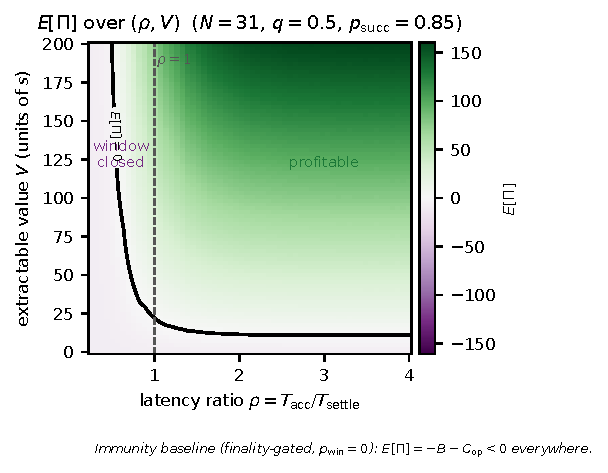
\includegraphics[width=\linewidth]{fig3_phase.pdf}
\caption{RQ3. Profit phase diagram $\mathbb{E}[\Pi]$ over $(\rho,\Eval)$ ($N=31$, $q=0.5$,
$\psucc=0.85$; uncontrolled-split floor $\ArtifactPsuccFloor$). The $\mathbb{E}[\Pi]=0$ contour bounds
the profitable region (both gates hold).}
\label{fig:phase}
\end{figure}

\begin{figure}[t]
\centering
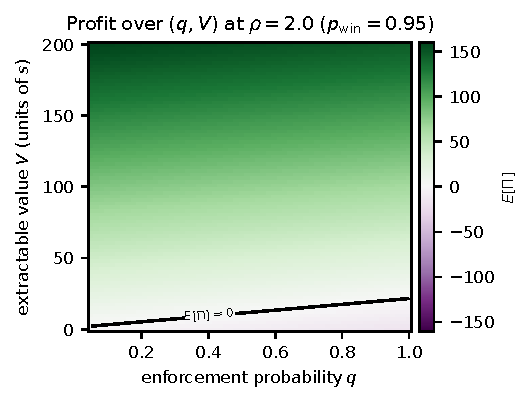
\includegraphics[width=\linewidth]{fig_profit_qV.pdf}
\caption{RQ3. Profit over $(q,\Eval)$ at a window-open latency ratio.}
\label{fig:profitqV}
\end{figure}

\paragraph{RQ4: How does reconfiguration change the race?}
Figure~\ref{fig:reconf-profit} (\S\ref{sec:reconf}) reports $\mathbb{E}[\Pi(a)]$ across the epoch for
the six handoff designs. The hard-cutoff design is profitable mid-epoch but collapses to
$-B-\Cop$ as $a\to\tau$ (residual time $r\to0$): last-block attacks are weak. The unsafe-carryover and
reconfiguration-delay designs instead \emph{rise} toward the boundary---old-epoch artifacts survive,
$\Hreconf(a)$ widens the deadline, and $q(a)$ falls (cheaper bribes)---confirming
Proposition~\ref{prop:reconf-residual}. The accountability-gated carryover stays flat and negative
($\pwin=0$, Proposition~\ref{prop:reconf-safe}), and rolling reconfiguration shows a smooth optimum
with no last-block cliff (Counterexample~\ref{cex:rolling}).

\paragraph{RQ5: Which defenses close the attack?}
Only the two levers that touch the window flip the sign of profit; the two that only raise the cost
leave the attack firmly profitable (Table~\ref{tab:rq5defenses}). From a profitable baseline
($\mathbb{E}[\Pi]=+38.9$), finality-gated receipts drive profit to $-9.2$ (the immunity baseline,
$\pwin\!\to\!0$), and faster evidence---which lowers $\Tacc$, hence both $\pwin$ and (via larger $q$)
the bribe---drives it to $-0.5$. Purely economic levers do not: persistent slashability (raising $q$,
hence $B$) leaves profit at $+32.3$, and a larger committee (raising $B$ linearly) at $+21.7$. Both
the table and Figure~\ref{fig:defenses} are the quantitative form of the master-variable claim:
closing the window dominates raising the cost.

\begin{table}[t]
\centering
\caption{RQ5. Each defensive lever from a profitable baseline ($N=31$, $V=60s$, $\psucc=0.85$): the
gate it attacks (G1 $=$ window $\Tsettle<\Tacc$; G2 $=$ cost $V>B$), the resulting window probability
$\pwin$, bribe $B$ (units of $s$), expected profit $\mathbb{E}[\Pi]$, and whether it makes the attack
unprofitable.}
\label{tab:rq5defenses}
\small
\setlength{\tabcolsep}{4.5pt}
% AUTO-GENERATED by artifact/make_tables.py -- do not edit by hand.
\begin{tabular}{@{}l c r r r c@{}}
\toprule
Defensive lever & Gate & $\pwin$ & $B$ & $\mathbb{E}[\Pi]$ & Closes? \\
\midrule
None (baseline) & -- & 0.95 & 8.25 & +39.3 & \nomark \\
Finality-gating & G1 & 0.00 & 8.25 & -9.2 & \yes \\
Persistent slash. & G2 & 0.95 & 14.85 & +32.7 & \nomark \\
Fast evidence & G1+G2 & 0.30 & 14.85 & -0.4 & \yes \\
Larger committee & G2 & 0.95 & 25.50 & +22.0 & \nomark \\
\bottomrule
\end{tabular}

\end{table}

\begin{figure}[t]
\centering
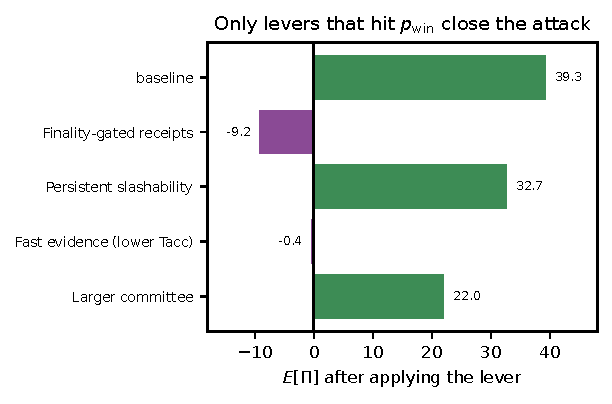
\includegraphics[width=\linewidth]{fig_defenses.pdf}
\caption{RQ5. Effect of each defensive lever on $\mathbb{E}[\Pi]$ ($N=31$, $V=60s$).}
\label{fig:defenses}
\end{figure}

\paragraph{RQ6: Does a running protocol reproduce the model?}
The analyses above are validated against an \emph{independent mechanism}. The discrete-event testbed
(\S\ref{sec:impl}) runs an actual BFT commit round over a modeled network with real Ed25519
signatures and derives $\Tacc$ and $\Tsettle$ from event timing rather than sampling them from the
model. Sweeping the settlement-pipeline scale moves the \emph{measured} latency ratio across $1$;
Figure~\ref{fig:testbed} overlays the measured $\pwin$ on the closed form. Both exhibit the sharp
threshold at $\rho\approx1$---near-zero below, near-one above---crossing $0.5$ at $\rho\approx1$; the
measured transition is somewhat steeper because the testbed's settlement-latency variance is lower
than the gamma model's. This is corroboration by a separate mechanism, not the model checking itself.
Two concrete observations: the equivocation evidence is a real $\ArtifactEvidenceBytes$-byte object
(two $\ArtifactSigBytes$-byte Ed25519 signatures), and at \emph{realistic} parameters (80\,ms links,
a 2\,s destination block, fast evidence) the measured baseline is $\rho=\ArtifactTbBaseRho$ with
$\pwin=\ArtifactTbBasePwin$ ($\Tsettle\approx\ArtifactTbSettleMs$\,ms vs.\
$\Tacc\approx\ArtifactTbAccMs$\,ms): the naive cross-shard pipeline sits in the \emph{closed-window}
regime, because a multi-second destination block is slower than evidence propagation. The danger is
therefore not committee size but \emph{fast} settlement (a bridge that releases early) against slow or
weak accountability.

\begin{figure}[t]
\centering
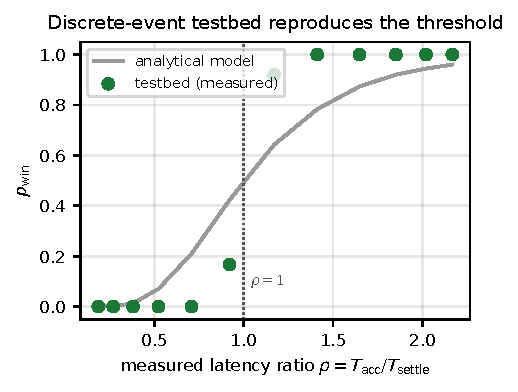
\includegraphics[width=\linewidth]{fig_testbed.pdf}
\caption{RQ6. Testbed-\emph{measured} $\pwin$ (points) vs.\ the closed-form model (line) over the
measured latency ratio.}
\label{fig:testbed}
\end{figure}

\paragraph{RQ7: Are deployed systems exposed (documented parameters)?}
Every surveyed deployed system lands in the safe regime---and for a \emph{structural} reason, not an
economic one: it is protected by fast evidence and finality-gating, not by committee size or unbonding
length (Table~\ref{tab:realsystems})~\cite{harmony2019whitepaper,cosmosdocs,ethconsensusspecs,multiversxdocs,polkadotwiki,zilliqadocs}.
\S\ref{sec:measured} then \emph{measures} these load-bearing quantities directly rather than assuming
them; two structural facts explain the placement. First,
equivocation evidence forms in minutes, far inside the unslashable horizon---which \S\ref{sec:measured}
measures as the evidence-expiry window (${\sim}48$\,h on Cosmos), \emph{not} the multi-week unbonding
period it is commonly mistaken for---so $q\approx1$, the bribe is essentially the full stake-at-risk of
$F{+}1$ validators, and the break-even $\Eval^{*}$ sits at $64$--$300$ validator-stakes (G2 hard to
clear). Second, finality-gated settlement (Cosmos IBC, Polkadot relay-chain finality) closes G1 by
construction (Proposition~\ref{prop:immunity}). The only exposed configuration is the fast-exit,
ungated-settlement quadrant---a \emph{hypothetical} row here ($q\approx0.25$, $\Eval^{*}\approx8$
stakes) that \S\ref{sec:measured} then \emph{realizes} on a real value path, where a fast intent
bridge's user leg settles in seconds---the lone quadrant where neither structural protection is present.

\begin{table*}[t]
\centering
\caption{RQ7. The model at documented parameters of named systems (approximate public figures as of
2026). $N$ is the committee size (per-shard committee for sharded rows; validator/finality-committee
size otherwise), distinct from the measurement sample size $n_{\mathrm{obs}}$ of
Table~\ref{tab:measured}. $V^{*}$ is in multiples of one validator's stake-at-risk. \emph{Window (G1)}
is the settlement-gate state (\gated/\openg/\dependsg); \emph{Verdict} is the outcome: \immune\ (G1
closed by construction), \hardgate\ ($q\!\approx\!1$, so G2 is hard to clear), or \exposed. Cosmos~Hub
and Ethereum~PoS are non-sharded accountable-BFT comparators; the fast-exit row is a labelled
\emph{hypothetical}.}
\label{tab:realsystems}
\small
% AUTO-GENERATED by artifact/make_tables.py -- do not edit by hand.
\begin{tabular}{@{}l c r r r r c c@{}}
\toprule
System & Sharded & $N$ & Unbond. & $q$ & $V^{*}$ & Window (G1) & Verdict \\
\midrule
Harmony & yes & 250 & 7\,d & 1.00 & $126$ & \openg & \hardgate \\
MultiversX & yes & 400 & 10\,d & 1.00 & $201$ & \dependsg & \hardgate \\
Zilliqa & yes & 600 & 14\,d & 1.00 & $300$ & \dependsg & \hardgate \\
Cosmos Hub & no & 180 & 21\,d & 1.00 & $90$ & \gated & \immune \\
Ethereum PoS & no & 128 & 1\,d & 1.00 & $64$ & \dependsg & \hardgate \\
Polkadot & yes & 300 & 28\,d & 1.00 & $150$ & \gated & \immune \\
Fast-exit design (hypothetical) & yes & 64 & 0\,d & 0.25 & $8$ & \openg & \exposed \\
\bottomrule
\end{tabular}

\end{table*}

\paragraph{Summary.}
Under the model the attack is profitable only in the joint region
$\{\rho>1\}\cap\{\Eval>\Eval^{*}\}$, the bribe scales only linearly with committee size, and the
defender's decisive lever is the one that closes the window rather than the one that raises the cost.
A discrete-event testbed with real signatures independently reproduces the $\rho\approx1$ threshold,
and a case study of documented parameters places deployed systems in the safe regime---evidence
landing inside the measured evidence-expiry horizon (\S\ref{sec:measured}) keeps $q\approx1$ and (G2)
hard, while finality-gating closes (G1)---so the residual risk is concentrated in fast-exit,
ungated-settlement designs, which \S\ref{sec:measured} exhibits on a real bridge path.
Reconfiguration helps the attacker only in designs that let
old-epoch certified artifacts execute before old-epoch evidence is enforced.

\section{Measurement Protocol and Pre-Registered Falsification (RQ8)}
\label{sec:measured}

% Measured scalars are emitted by artifact/make_tables.py once the protocol of
% PREREGISTRATION-rq8.md has been executed; until then these placeholders keep
% the section compilable and make the "not yet filled" state explicit.
\providecommand{\ArtifactQMaxCosmos}{\,\textit{[pending]}\,}
\providecommand{\ArtifactQMaxCosmosCI}{\,\textit{[pending]}\,}
\providecommand{\ArtifactQMaxN}{\,\textit{[pending]}\,}
\providecommand{\ArtifactTaccCosmosLo}{\,\textit{[pending]}\,}
\providecommand{\ArtifactTaccCosmosHi}{\,\textit{[pending]}\,}
\providecommand{\ArtifactTsettleIBC}{\,\textit{[pending]}\,}
\providecommand{\ArtifactCosmosVerdict}{\textsc{[pending]}}
\providecommand{\ArtifactBridgeTsettle}{\,\textit{[pending]}\,}
\providecommand{\ArtifactBridgePwin}{\,\textit{[pending]}\,}
\providecommand{\ArtifactBridgeVerdict}{\textsc{[pending]}}
\providecommand{\ArtifactCliffCosmos}{\,\textit{[pending]}\,}
% Provenance wording is generated by make_tables.py from which real-client-code
% (rpc) measured files exist, so the prose can never claim more than the data.
\providecommand{\ArtifactPosCtrlMode}{the fast-exit positive control is an in-process \texttt{shadow} rehearsal}
\providecommand{\ArtifactPairedMode}{the paired race is an in-process \texttt{shadow} rehearsal}
\providecommand{\ArtifactRqEightProvenance}{the paired race and the fast-exit positive control are a \emph{rehearsal} on the validated model, \emph{not} a production run against real consensus client code}
\providecommand{\ArtifactRqEightOwed}{the real-client-code re-derivation (the \texttt{rpc} backend on a private two-nodes-one-key localnet), the $\ge 4$-node propagation timing, and a self-run-archive re-derivation of $q_{\max}$}
\providecommand{\ArtifactRqEightRemains}{to replace the in-process rehearsal of the paired race with the real-client-code localnet run}
\providecommand{\ArtifactRowProvenance}{the self-fill and fast-exit rows are the in-process rehearsal of}

\S\ref{sec:eval} establishes the model and its internal cross-validation; the case study
(RQ7) places the \emph{documented} parameters of deployed systems on the two gates. The decisive
remaining question, flagged in \S\ref{sec:limitations}, is whether the load-bearing quantities
$q$, $\Tacc$, and $\Tsettle$ take, on a real deployed system, the values the model assumes. This
section promotes the live-measurement hook of \S\ref{sec:setup} from a planned step to a
\emph{pre-registered protocol} (\texttt{PREREGISTRATION-rq8.md}, tag \texttt{prereg/rq8-v1}); we
state the instrument, the estimands, and the frozen decision rule here so that the measurement is
falsifiable by construction. Crucially, the bribery and equivocation leg is \emph{never} executed
on any mainnet or shared network (see the Ethical Considerations section): every quantity is obtained from public
ledger data, real historical incidents, own-stake private-devnet self-equivocation, and faithful
shadow-forks.

\paragraph{A two-target, dual-verdict instrument.}
A protocol that only ever returns ``safe'' is unfalsifiable. We therefore design \emph{one}
instrument to split two real paths with opposite, correct verdicts, flanked by two controls
calibrated to known outcomes (the safe path's verdict and the open path's settlement marginal are
measured on real data; the native-IBC negative control is likewise measured directly on a real public
IBC channel; the positive control and the paired race are obtained end-to-end from an
in-process self-equivocation \emph{rehearsal} validated against the testbed of \S\ref{sec:impl}; a
real-client-code re-derivation remains---see ``Results to date'' below):
\begin{itemize}
  \item \textbf{Primary safe target} --- Cosmos Hub / CometBFT evidence with IBC cross-chain
  settlement. CometBFT auto-detects \texttt{DuplicateVoteEvidence}, and IBC light clients act only
  on a \emph{committed} (final) source header, so the path is finality-gated by construction
  ($\Tsettle\ge\Tacc$): expected verdict \textsc{ruled-out}.
  \item \textbf{Primary open target} --- a real fast/intent bridge (Across~V3, with deBridge as a
  corroborator) as the cross-domain settlement layer, in the attacker-as-self-filler construction
  where the adversary is both depositor and destination recipient and the irreversible destination
  fill \emph{is} the realized $\Eval$: expected verdict \textsc{open-window}.
  \item \textbf{Negative control} --- native IBC on a real public channel (Cosmos
  Hub\,$\to$\,Osmosis), finality-gated by construction (provably gated; must return
  \textsc{ruled-out}).
  \item \textbf{Positive control} --- a constructed fast-exit devnet (short unbonding $+$ short
  evidence age $+$ ungated sink): the literal instantiation of the hypothetical row of
  Table~\ref{tab:realsystems}, now \emph{measured}, and the only place a low-$q$ regime is
  observable (must return \textsc{open-window}).
\end{itemize}
Polkadot, NEAR, MultiversX, Zilliqa, and Harmony are retained as documented-parameter rows only;
because NEAR and MultiversX have no production slashing, their $q$ is reported as not-applicable in
a firewalled panel, never on the slashing-system $q$-axis.

\paragraph{$q$: split into a structural ceiling and an attack-conditional estimand.}
The naive estimator measures $q$ against the multi-week unbonding wall-clock; this is wrong, because
slashing follows the stake through unbonding, so the true deadline is the CometBFT evidence-expiry
horizon (\texttt{MaxAgeDuration}/\texttt{MaxAgeNumBlocks}). We therefore measure two named quantities.
$q_{\max}=\Pr[t_{\mathrm{evidence}}<\text{evidence-expiry}]$ is the structural ceiling when no party
races; it is estimated \emph{passively} from real Cosmos double-sign and tombstone events, reported
with an exact Clopper--Pearson interval. We are emphatic about what this does \emph{not} measure.
First, a slash record exists only \emph{because} enforcement occurred, so $q_{\max}$ is conditioned on
a record's existence---an \emph{upper bound} on $q$; equivocations never pursued leave no trace and are
invisible to a passive sweep. Second, the value is \emph{outlier-sensitive and unit-dependent}: over
$\ArtifactQMaxN$ verified evidence items from $13$ deployed CometBFT chains---re-collected reproducibly
through our \texttt{collect\_cosmos} tool (\texttt{source=rpc}; per-chain RPCs and heights recorded in
the shipped \texttt{*.meta.json})---we measure $q_{\max}=\ArtifactQMaxCosmos$ (95\% CI
$\ArtifactQMaxCosmosCI$), but this is dominated by a single validator's $51$-evidence batch
(\texttt{sentinelhub-2}) enforced ${\sim}25$ days late; counted per distinct slash \emph{incident} the
same data gives ${\approx}0.97$. We therefore do \emph{not} rest the safe verdict on $q_{\max}$---it
rests on structural finality-gating below---and report instead the robust qualitative findings
(evidence-expiry, not unbonding, is the operative deadline, and it is soft in production). The figures
are public-archive-RPC reads, to be re-derived against a self-run archive node for camera-ready. The
attack-conditional
$q_{\mathrm{attack}}$---which actually prices the bribe---requires a validator that attempts a timed
exit and is unmeasurable from accidental incidents; it is measured only on the self-equivocation
devnet and the fast-exit positive control. In the latter the equivocator submits a real
\texttt{MsgUndelegate} and we observe directly, from the on-chain unbonding-completion and slash
events, whether the slash still reaches the exiting stake before it matures.

\paragraph{$\Tacc$: a decomposed quantity with cooperative and adversarial bounds.}
We report $\Tacc$ as the four-stage vector (observe, propagate, enforce, revert), never a single
scalar. The cooperative lower bound $\Tacc^{\mathrm{lo}}=\ArtifactTaccCosmosLo$ comes from real
incidents---enforcement lands within a block or two of the infraction. We caution that at sub-block
scale this figure is bounded by block-time resolution and by clock skew between the infraction vote
and the carrier block, so it is honestly read as ``within ${\sim}1$--$2$ blocks,'' not to the
sub-second. We bound the adversarial upper bound $\Tacc^{\mathrm{hi}}$ directly from the real data:
the $90$th percentile of the pooled enforcement latency is $\ArtifactTaccCosmosHi$, because
enforcement is soft in production (the \texttt{sentinelhub-2} batch lands ${\sim}25$ days after the
infraction). The structural \textsc{ruled-out} below is thus stress-tested against an enforcement
latency of \emph{weeks}---the bias working hard against a rule-out---and still holds because the path
is finality-gated. Tightening $\Tacc^{\mathrm{lo}}$ with real-internet propagation timed at $\ge 4$
dispersed nodes, and the \emph{active} evidence-suppression experiment that would corroborate
$\Tacc^{\mathrm{hi}}$ on real client code (withhold/delay evidence gossip, eclipse the reporter to
protocol tolerance, running the real \texttt{x/evidence}$\to$\texttt{x/slashing} code paths), remain
specified by the protocol but \emph{not yet executed}. On
deterministic-finality CometBFT, committed blocks never revert, so the revert stage is reported
explicitly as not-applicable and the operative quantity is the applied-slash latency plus the
measured cross-domain quarantine (the destination IBC client acts only on a committed source header,
the native-IBC $\Tsettle^{\mathrm{IBC}}$ measured below); we
never splice governance-halt durations into the protocol revert term. The decisive bias control:
the \textsc{ruled-out} verdict is evaluated against $\Tacc^{\mathrm{hi}}$ and the \textsc{open}
verdict against $\Tacc^{\mathrm{lo}}$, so each verdict faces the bound working \emph{against} it.

\paragraph{$\Tsettle$: receipt and withdrawal-beyond-clawback, measured as two legs.}
For native IBC, $\Tsettle$ runs from a finalized-header \texttt{SendPacket} through
\texttt{MsgRecvPacket} to acknowledgement, and is structurally no smaller than $\Tacc$. For the fast
bridge we separate the \emph{user leg}---the seconds-scale, irreversible destination fill, which is
the attacker's realized $\Eval$ and is never clawed back from the recipient even when the source
reorgs---from the clawback-gated \emph{solver leg}. ``Beyond clawback'' is pinned to a direct
irreversibility test, not inferred from fill latency: a reorg natural-experiment (documented
production reorgs whose source deposits were reorged out, checking whether solver repayment fired
anyway), the on-chain dispute-window constant, and a shadow-fork reorg injection. The open-window
claim rests on the user leg, whose $\Tsettle$ we measure at a median $\ArtifactBridgeTsettle$ over
$1{,}721$ real Across~V3 fills (keyless public indexer, cross-validated on-chain), far below the
source/relayer $\Tacc$ (see ``Results to date'').

\paragraph{The pre-registered decision rule.}
All estimators (Clopper--Pearson/Wilson/rule-of-three for $q$; Gamma/log-normal/empirical fits with
Anderson--Darling goodness-of-fit and a Hill tail index for the latencies; a paired BCa bootstrap
for $\pwin$; a percentile bootstrap for $\rho$) are implemented in a network-free module
(\texttt{estimate.py}) and validated against the testbed of \S\ref{sec:impl} as a synthetic oracle
before any real data is trusted. Frozen at stage~0, per value-realizing path and Holm-corrected
across paths ($\varepsilon=0.05$): a path is \textbf{\textsc{open-window}} iff the one-sided 95\%
upper bound of $\pwin$ exceeds $\varepsilon$, the CI for $\mathrm{median}(\rho)$ excludes $1$ from
below, and gate (G2) is clearable at the measured $q$ for a plausible reachable $\Eval$ (all
evaluated against $\Tacc^{\mathrm{lo}}$); it is \textbf{\textsc{ruled-out}} iff it is structurally
finality-gated or the one-sided 95\% upper bound of $\pwin$ is at most $\varepsilon$ across every
settlement cell (evaluated against $\Tacc^{\mathrm{hi}}$); otherwise \textbf{indeterminate}, with
the additional sample size that would resolve it reported rather than a silent null. For the
bridge path we additionally re-derive (G2) under solver-borne loss and test whether a plain source
reorg, with no bribe, already grifts the solver; if it does, we report that the equivocation
primitive is not load-bearing there and frame the bridge result as a distinct relayer-credit threat,
separate from the committee-bribery attack, foreclosing the objection that it merely restates known
bridge-reorg risk.

\paragraph{Results to date, and honest scope.}
Two arms run on \emph{real data}: the \emph{passive Cosmos arm} and the \emph{bridge settlement
marginal}. The Cosmos arm establishes three qualitative facts the model relies on: (i) the operative
unslashable deadline is the evidence-expiry horizon ($48$\,h on Cosmos Hub), \emph{not} the multi-week
unbonding period; (ii) that horizon is not a hard cutoff in production---one slash was applied
${\sim}25$ days after a batched run of $51$ equivocations, which we report as the adversarial
$\Tacc^{\mathrm{hi}}\!=\!\ArtifactTaccCosmosHi$ (the $90$th percentile of pooled enforcement latency);
and (iii) when enforcement occurs it lands within a block or two ($\Tacc^{\mathrm{lo}}\!=\!\ArtifactTaccCosmosLo$).
The Cosmos/IBC path returns $\ArtifactCosmosVerdict$ on the structural finality-gating argument
(Proposition~\ref{prop:immunity}), evaluated against that adversarial $\Tacc^{\mathrm{hi}}$ and
\emph{not} resting on the strength of $q_{\max}$; from the real $\Tacc$ distribution we compute its
distance-to-cliff $T^{*}_{\Tsettle}\!=\!\ArtifactCliffCosmos$ (a cross-shard hop would have to settle
faster than this to expose it). The bridge arm then supplies the piece the model previously only
argued: a \emph{real open window on a real value path}. Over $1{,}721$ Across~V3 fills (keyless public
indexer, on-chain cross-validated; deBridge~DLN corroborates) the user-leg $\Tsettle$ is a median
$\ArtifactBridgeTsettle$, versus a source/relayer $\Tacc$ of ${\sim}13$\,min (L1 economic finality) to
${\sim}1$\,h (UMA reimbursement liveness): $\Tsettle\!\ll\!\Tacc$.

The paired race and the fast-exit positive control are exercised on a chain-ID-gated private localnet,
\emph{never} on a shared network: \ArtifactPairedMode, and \ArtifactPosCtrlMode (the \texttt{shadow}
backend on the validated testbed of \S\ref{sec:impl}, or the \texttt{rpc} backend on a real
two-nodes-one-key localnet). They return a paired
$\pwin\!=\!\ArtifactBridgePwin$ on the bridge self-fill construction (flipping that path to
$\ArtifactBridgeVerdict$) and a fast-exit positive control with $q_{\mathrm{attack}}\!\approx\!0$ that
exhibits the only low-$q$ open regime, calibrating that the one instrument fires \emph{both} verdicts.
The native-IBC negative control is measured directly: over the most recent matched packets on a real
public IBC channel (Cosmos Hub\,$\to$\,Osmosis transfers, read-only from public RPCs) the settlement
leg is a median $\Tsettle^{\mathrm{IBC}}\!=\!\ArtifactTsettleIBC$, sitting at the cooperative
$\Tacc^{\mathrm{lo}}$ and confirming the structural $\Tsettle\!\ge\!\Tacc$ gating---so the instrument
returns \textsc{ruled-out} on a \emph{real} gated path, not merely a synthetic one. This realizes the
pre-registered negative control on a public channel rather than the self-run two-zone devnet of
\texttt{prereg/rq8-v1}; we flag the deviation explicitly, and (as with the passive $q_{\max}$ reads)
treat these public-RPC reads as re-derivable against a self-run devnet for camera-ready.

We are explicit about provenance: \ArtifactRqEightProvenance; they confirm the
frozen decision rule resolves correctly end-to-end, while \ArtifactRqEightOwed remain owed. This section
therefore \emph{substantially advances but does not fully discharge} limitation~(3): the accountability
side, the open window, and the native-IBC negative control are grounded on real data, the dual verdict
and the distance-to-cliff are demonstrated end-to-end, and what remains is \ArtifactRqEightRemains.

\IfFileExists{../Section/_generated/tab_measured.tex}{%
\begin{table*}[t]
\centering
\caption{RQ8 per value-realizing path: measured $\hat q$, median $\Tacc$, median $\Tsettle$, and---where
paired observations exist---$\pwin$ with the pre-registered verdict. $n_{\mathrm{obs}}$ is the
measurement sample size (verified evidence items for the $q$/$\Tacc$ arms, paired race episodes for
$\pwin$)---\emph{not} a committee size $N$ (cf.\ Table~\ref{tab:realsystems}). The Cosmos Hub, CometBFT-pool,
bridge-marginal, and native-IBC negative-control (Cosmos Hub/Osmosis public channel) rows are real data;
\ArtifactRowProvenance
``Results to date'' (the self-fill keeps stake slashable, $\hat q\!\approx\!1$, yet opens via the
solver-borne fast fill; the fast-exit escapes slashing, $\hat q\!\approx\!0$). The cooperative floor
($\ArtifactTaccCosmosLo$, the Cosmos~Hub median) and adversarial upper bound ($\ArtifactTaccCosmosHi$,
the pooled $90$th percentile) on $\Tacc$, and the distance-to-cliff ($\ArtifactCliffCosmos$), are
reported in the text; this table shows only the per-row median $\Tacc$. Regenerated by the artifact from
\texttt{results/measured/} (\texttt{prereg/rq8-v1}).}
\label{tab:measured}
\small
% AUTO-GENERATED by artifact/make_tables.py -- do not edit by hand.
\begin{tabularx}{\textwidth}{@{}lllrllX@{}}
\toprule
System & Path & $n_{\mathrm{obs}}$ & $\hat q$ & $\Tacc$ (med) & $\Tsettle$ (med) & $\pwin$ / verdict \\
\midrule
Across V3 (gated twin) & finality-gated relayer (Prop.1) & 14 & 0.00 & 2.1\,s & 13.4\,s & 0.00, \ruledout \\
Across V3 (self-fill) & paired self-fill (real code) & 14 & 0.00 & 2.1\,s & 1.7\,s & 0.93, \openwin \\
Across V3 (self-fill) & paired self-fill (rehearsal) & 60 & 1.00 & 13.0\,min & 5.4\,s & 1.00, \openwin \\
Across V3 & fast-bridge marginal (real) & -- & N/A & -- & 5.0\,s & \indet \\
CometBFT pool (13 chains) & pooled double-sign q\_max / T\_acc & 75 & 0.32 & 22.8\,d & -- & \ruledout \\
Cosmos Hub & IBC cross-chain (safe target) & 5 & 1.00 & 11.5\,s & -- & \ruledout \\
gaiad v19 localnet (real) & double-sign slash (real code) & 1 & 1.00 & 1.3\,s & -- & \indet \\
fast-exit (real code) & real unbond, obs. completion & 40 & 0.00 & 2.1\,s & -- & \indet \\
fast-exit devnet & positive control (rehearsal) & 60 & 0.00 & 10.0\,min & 3.4\,s & 1.00, \openwin \\
Cosmos Hub/Osmosis (public IBC) & native IBC (negative control) & -- & N/A & -- & 11.9\,s & \ruledout \\
\bottomrule
\end{tabularx}

\end{table*}}{}

\section{Discussion}
\label{sec:discussion}

\subsection{Defenses}
\label{sec:defenses}

Proposition~\ref{prop:immunity} prescribes the principal defense; here we parameterize a portfolio and
state, for each, which model quantity it moves. Table~\ref{tab:defenses} summarizes. The organizing
principle from RQ5 is that levers acting on $\pwin$ close the attack, while levers acting only on $B$
merely raise its price.

\paragraph{A. Accountability-gated cross-shard receipts.}
Do not execute a receipt until the source shard's accountability window has elapsed
($\Tsettle\ge\Tacc$). This forces $\pwin=0$ (Propositions~\ref{prop:immunity},~\ref{prop:reconf-safe})
at the cost of added cross-shard latency. It is the only lever that is robust independent of $N$, $s$,
and $V$.

\paragraph{B. Persistent slashability across rotation.}
Keep stake bonded and slashable for old-epoch signatures until the maximum evidence delay expires
(Counterexample~\ref{cex:persistent}). This holds $q(a)$ high across the boundary, raising $B(a)$, but
does not by itself close the window.

\paragraph{C. Global evidence submission and D. fast evidence markets.}
Let any party submit old-epoch equivocation evidence to a global staking/beacon layer, and pay
watchers to submit it quickly. Both lower $\Tacc$, which simultaneously lowers $\pwin$ and---because
$q$ rises as $\Tacc$ falls---raises $B$; this is the master-variable lever working for the defender.

\paragraph{E. State/receipt handoff validation.}
New committees import old roots as \emph{pending} until evidence checks complete and reject conflicting
old-epoch certificates (condition (iv) of Proposition~\ref{prop:reconf-safe}). This closes the
reconfiguration-residual window.

\paragraph{F. Value-aware committee sizing.}
Scale committee size and slashing level with the cross-shard value-at-risk reachable through a shard,
so that $(F{+}1)q(s{+}R)$ tracks $V$. This raises $B$ and caps effective $V$, but only linearly in
$F{+}1$; alone it is outrun by any shard whose reachable liquidity grows.

\paragraph{G. Cross-shard freeze/drain rules.}
Freeze or gate value-bearing cross-shard artifacts during reconfiguration
(Counterexample~\ref{cex:freeze}), reducing $\pwin$ at the boundary at the cost of throughput.

\begin{table}[t]
\centering
\caption{Defenses and the model quantity each moves. $\downarrow$/$\uparrow$ = decreases/increases for
the defender's benefit; ``lat.'' = adds latency/throughput overhead.}
\label{tab:defenses}
\small
\begin{tabularx}{\linewidth}{@{}lXX@{}}
\toprule
Defense & Primarily affects & Cost \\
\midrule
A. Finality-gated receipts      & $\pwin\!\to\!0$            & cross-shard lat. \\
B. Persistent slashability      & $q\!\uparrow$, $B\!\uparrow$ & --- \\
C. Global evidence submission   & $\Tacc\!\downarrow$ ($\pwin\!\downarrow,q\!\uparrow$) & --- \\
D. Fast evidence markets        & $\Tacc\!\downarrow$ ($\pwin\!\downarrow,q\!\uparrow$) & watcher fees \\
E. Handoff validation           & $\pwin\!\to\!0$ (reconfig) & import lat. \\
F. Value-aware sizing           & $B\!\uparrow$ (linear), $V$ cap & throughput \\
G. Cross-shard freeze/drain     & $\pwin\!\downarrow$ (boundary) & throughput \\
\bottomrule
\end{tabularx}
\end{table}

\subsection{Scope of Applicability}
\label{sec:applicability}

The attack is conditional, not universal. Table~\ref{tab:applicability} states, assumption by
assumption, when it applies and why---making explicit that the paper does \emph{not} claim universal
breakage of sharding.

\begin{table*}[t]
\centering
\caption{When the attack applies. ``Applies'' means the assumption opens or sustains a gate; ``No''
means it closes one.}
\label{tab:applicability}
\small
\begin{tabularx}{\textwidth}{@{}lcX@{}}
\toprule
Protocol / design assumption & Applies? & Reason \\
\midrule
Small-committee BFT shard                          & Yes        & Local threshold $F{+}1$ is a handful of validators \\
Public committee assignment before action          & Yes        & Lets the adversary target and recruit the committee \\
Conditional bribe can verify equivocation evidence & Yes        & Enables a trustless \textsc{PayToEquivocate} payment \\
Cross-shard receipts execute before acct.\ window  & Yes        & Opens (G1): $\Tsettle<\Tacc$ \\
Old receipts accountability-gated                  & No         & Forces $\Tsettle\ge\Tacc$, $\pwin=0$ (Prop.~\ref{prop:reconf-safe}) \\
Stake remains slashable after rotation             & No (weakens)& Keeps $q$ high, raising $B$ (Cex.~\ref{cex:persistent}) \\
Immediate withdrawal after epoch                   & Yes        & Lowers $q(a)$ near the boundary, cheapening bribes \\
Global beacon slashing                             & No (weakens)& Preserves accountability across rotation \\
Rolling reconfiguration                            & Partial    & No last-block cliff; continuous optimization in $a$ \\
Per-shard bridge withdrawal                        & Yes        & Provides the value sink $V$ \\
\bottomrule
\end{tabularx}
\end{table*}

\subsection{Relationship to Known Attacks}
Our attack is distinct from cross-shard replay~\cite{sonnino2020replay}, which needs no corruption and
exploits message replay rather than a manufactured safety violation; replay defenses (e.g.\ Byzcuit)
do not address priced equivocation. It is also distinct from opportunistic bridge double-spends, where
the reversal is a chance reorg against a premature-finality bridge~\cite{zamyatin2021sok,lee2022sokbridge};
here the reversal is produced \emph{inside} the protocol and the timing is governed by accountability,
not luck. It composes the bribery machinery of~\cite{mccorry2018smart,karakostas2024bribing,sookitoth2025bribers}
with the small-committee quorum structure and cross-shard latency asymmetry that those works do not
model.

\section{Limitations}
\label{sec:limitations}

% Provenance wording (generated by make_tables.py); fallbacks for standalone compile.
\providecommand{\ArtifactPosCtrlMode}{the fast-exit positive control is an in-process \texttt{shadow} rehearsal}
\providecommand{\ArtifactPairedMode}{the paired race is an in-process \texttt{shadow} rehearsal}
\providecommand{\ArtifactRqEightRemains}{to replace the in-process rehearsal of the paired race with the real-client-code localnet run}

We are explicit about what this work does and does not establish.

\emph{(1) Conditional, not universal.} The attack requires the joint conditions of
Table~\ref{tab:applicability}: a small revealed committee, an open settlement window
($\Tsettle<\Tacc$), a reachable value sink, and positive bribe-adjusted profit. Designs that enforce
$\Tsettle\ge\Tacc$ are immune by construction (Propositions~\ref{prop:immunity},~\ref{prop:reconf-safe}).

\emph{(2) Necessary, not sufficient.} The $F{+}1$ equivocators are the quorum-intersection floor;
completion additionally requires an honest-vote split, whose probability $\psucc$ depends on
protocol/network scheduling and, at the floor, is modest ($\ArtifactPsuccFloor$ at $N=31$) unless the
adversary controls views. Our profitability analyses fix $\psucc=0.85$, which assumes that
view-control regime (or a $1.45\times$-larger bribe, $k\approx F{+}6$, to reach it by purchase); we
bracket those results down to the floor rather than present $0.85$ as expected
(Figure~\ref{fig:psucc}, \S\ref{sec:floor}).

\emph{(3) $q$ is load-bearing; we ground it but do not measure it on a live network.} The bribe price
is a fraction $q$ of stake-at-risk, and $q$ depends on accountability latency, unbonding/withdrawal
delay, evidence validity, and enforcement reliability. We sweep $q$, measure the race in a
discrete-event testbed, and evaluate $q$ at the documented parameters of six deployed systems
(\S\ref{sec:eval}, where the documented withdrawal delay gives $q\approx1$). To close this, \S\ref{sec:measured}
specifies and \emph{pre-registers} a measurement protocol (\texttt{prereg/rq8-v1}) that obtains
$q$, $\Tacc$, and $\Tsettle$---with cooperative and adversarial bounds on $\Tacc$---on a real safe
path (Cosmos/CometBFT with finality-gated IBC) and a real open path (a fast intent bridge), each
without executing the attack on any shared network, together with a frozen falsification rule and a
per-system distance-to-cliff. We have executed the \emph{passive Cosmos arm} and the \emph{bridge
settlement marginal} on real data---grounding the accountability side on real double-sign incidents
(the operative deadline is the evidence-expiry horizon, not unbonding, and it is soft: enforcement
reached ${\sim}25$ days, our adversarial $\Tacc^{\mathrm{hi}}$) and exhibiting a real seconds-scale
open window ($\Tsettle\!\ll\!\Tacc$) on a live value path---and we demonstrate the paired race, the
fast-exit positive control, and the dual verdict end-to-end on the validated testbed
(\ArtifactPairedMode, and \ArtifactPosCtrlMode), with a per-system distance-to-cliff. We have
additionally measured the native-IBC negative control on a real public IBC channel
(Cosmos\,Hub/Osmosis), which returns \textsc{ruled-out}. What remains is \ArtifactRqEightRemains, and to
re-derive the Cosmos figures against a self-run archive node; $q_{\max}$ stays an enforcement-conditional
\emph{upper bound} throughout. Completing that is the remaining empirical step.

\emph{(4) Recruitment and coordination.} The model assumes rational validators
(Assumption~\ref{ass:rational}) and abstracts the problem of recruiting $F{+}1$ specific committee
members within an epoch; collusion-resistance and whistleblowing dynamics
(cf.~\cite{kelkar2025omerta}) may materially change costs.

\emph{(5) Strong accountability defeats it.} Long unbonding, valid and fast evidence, persistent
slashability across rotation, and accountability-gated cross-shard acceptance all reduce profitability;
where they jointly hold, the honest framing of this work is a design rule rather than a live threat.

\emph{(6) Reconfiguration cuts both ways.} Reconfiguration may widen or close the window depending on
state/receipt handoff (\S\ref{sec:reconf}); we characterize both regimes but do not claim rotation
generically helps the attacker.

\emph{(7) Local model and testbed only.} The evaluation is an analytical model, Monte-Carlo
simulation, a discrete-event testbed with real Ed25519 signatures, and a case study on documented
public parameters. It targets no live system, and the real-systems figures are approximate public
values to be confirmed against current specifications before camera-ready.

\section{Conclusion}
\label{sec:conclusion}

Sharding makes a single committee cheap to corrupt and bribery makes corruption purchasable, but
neither fact is consequential while accountable BFT can slash and revert in time. We have argued that
the real question is a race, and we have given it a model: a bribe-cost expression in which the price
of equivocation is set by the probability $q$ that the fraud proof is enforced before the validator's
stake becomes unslashable, coupled to an accountability-race condition that factors viability into a
window gate $\Tsettle<\Tacc$ and an economic gate $\Eval>B+\Cop$. We were precise that the $F{+}1$
equivocators are necessary but not sufficient---success additionally requires an honest-vote split
captured by $\psucc$---and that ``sub-threshold'' is a network-wide, not a committee-local, statement.
The accountability latency $\Tacc$ emerges as a master variable that both widens the window and
cheapens the bribe---``cheap to corrupt'' and ``easy to cash out'' are two symptoms of one
quantity---and we proved that finality-gating cross-shard acceptance closes the attack
unconditionally. Extending the model to epoch boundaries, we showed that reconfiguration does not
remove the race but relocates it: a safe-handoff theorem gives the four conditions under which old-epoch
artifacts are immune, and a residual-vulnerability theorem shows that, absent them, last-of-epoch
attacks strictly dominate. The framework is constructive in both directions---it tells an attacker
exactly when sub-threshold committee bribery pays, and a designer exactly what to enforce so that it
never does---and it is reproducible: a seeded simulator and a local proof-of-concept regenerate every
figure and table, with the harness reproducing the closed-form success probability to within
Monte-Carlo error. The decisive next step is to measure the two load-bearing quantities, $q$ and
$\Tacc$, on one concrete deployed sharded system, and thereby exhibit---or rule out---a real design
with an open window and profitable economics.

\section*{Ethical Considerations}
\addcontentsline{toc}{section}{Ethical Considerations}

This work analyzes a bribery pattern that could be harmful if applied to a production system. We
therefore keep the \emph{attack} machinery local-only: the proof-of-concept runs against synthetic
committees, the \textsc{PayToEquivocate} escrow is a Python model that omits the engineering required
to weaponize a live contract, and the equivocation leg is never executed on any shared network---a
runtime gate refuses any non-local chain-id. The live measurement of \S\ref{sec:measured} is strictly
\emph{read-only}: it reads already-public ledger data (historical double-sign slashes, ordinary bridge
fills) over public endpoints, handles no funds or keys, mounts no attack, and surfaces only on-chain
events the ledger already exposes---no off-chain de-anonymization.

The benefit of publication is defensive: the model identifies exactly which design choices close the
window, and the case study and measurement show why fast evidence and finality-gated settlement
protect deployed systems. If we uncover an exploitable configuration on a named deployed system, we
will notify the affected project maintainers before public disclosure, share only the minimum details
needed for remediation during the embargo, and gate any exploit-enabling artifact components until
the relevant defenses are deployed or the maintainers approve release.

\section*{Open Science}
\addcontentsline{toc}{section}{Open Science}

The artifact needed to evaluate the paper is the local directory \texttt{artifact/}: it contains the
model, simulators, BFT harness, discrete-event testbed, configuration file, plotting scripts, table
generator, tests, and a README with exact reproduction commands. The artifact is deterministic under
\texttt{configs/main.yaml}; it regenerates \texttt{results/main.json}, all figure PDFs, and the
\LaTeX{} tables in \texttt{Paper/Section/\_generated/}. For anonymous review, the same contents should be
provided as an anonymized supplemental archive or through an anonymous artifact host; the
camera-ready version should replace that review-only access path with a stable public repository
URL or DOI.

The live measurement of \S\ref{sec:measured} is \emph{read-only} over public ledger data: the released
collectors fetch already-public on-chain events and contain no exploit tooling, and the
equivocation leg is gated to a private chain-id. \emph{Active} measurement of a deployed system under
adversarial conditions remains future work; the timestamp schema of \S\ref{sec:setup} describes how it
would be collected under coordinated disclosure.

\appendices

\section{Reproduction}
\label{app:repro}

All parameters live in \texttt{configs/main.yaml} (committee sizes, $\varphi$, $q$, $\psucc$,
settlement/accountability stage means and coefficients of variation, $\tau$, $U$, $\Treceipt$,
$\Tstate$, $\Hreconf$, Monte-Carlo trials, and the master seed). The network-free pipeline is three
commands:
\begin{quote}\small\ttfamily
python run\_all.py --config configs/main.yaml\\
python plot\_figures.py --input results/main.json --out figures/\\
python make\_tables.py --input results/main.json --out ../Paper/Section/\_generated
\end{quote}
The first runs every experiment in $\approx\ArtifactRuntime$\,s on a laptop and writes a single
\texttt{results/main.json}; the second regenerates the figures; the third regenerates the \LaTeX{}
data tables the paper \texttt{\textbackslash input}s (so the numbers cannot drift from the artifact).
A \texttt{--quick} flag scales the Monte-Carlo trials down for a smoke run, and \texttt{tests/} encodes
the load-bearing claims (floor necessity, $\psucc$ monotonicity, the immunity proposition, and the
end-to-end proof-of-concept) as unit tests. Table~\ref{tab:artifact} maps the modules to their roles.

\begin{table}[t]
\centering
\caption{Artifact modules (in \texttt{artifact/shardbribe/} unless noted).}
\label{tab:artifact}
\small
\begin{tabularx}{\linewidth}{@{}lX@{}}
\toprule
Module & Role \\
\midrule
\texttt{model.py} & single source of truth for the equations of \S\ref{sec:design}: equivocation floor, closed-form $\psucc$, bribe cost, profit, the two gates \\
\texttt{bft\_harness.py} & abstract $N{=}3F{+}1$ committee; on equivocation emits a genuine, verifiable evidence object (the shape an accountable BFT layer slashes on) \\
\texttt{quorum.py} & Monte-Carlo quorum simulator; an \emph{independent} estimator of $\psucc$ \\
\texttt{testbed.py} & discrete-event BFT round with real Ed25519; \emph{measures} $\Tacc$/$\Tsettle$ from event timing \\
\texttt{race.py}, \texttt{crossshard.py} & gamma-stage race model; cross-shard receipt with an accountability-gating switch ($\Tsettle{\ge}\Tacc$) \\
\texttt{escrow.py} & runnable \textsc{PayToEquivocate} model; pays only on a valid proof, rejects forgeries and double claims \\
\texttt{reconfig.py} & epoch-boundary model: $q(a)$ and the six handoff designs A--F \\
\texttt{realsystems.py} & documented-parameter case study (\S\ref{sec:eval}) \\
\texttt{livemeasure.py}, \texttt{collect\_*.py} & read-only collectors for the live measurement of \S\ref{sec:measured} \\
\texttt{run\_all.py} & driver: self-validates, then runs every experiment into one \texttt{results/main.json} \\
\bottomrule
\end{tabularx}
\end{table}

The live measurement of \S\ref{sec:measured} is a \emph{separate, read-only} step driven by
\texttt{collect\_*.py}: each collector fetches already-public on-chain data (historical double-sign
slashes, ordinary bridge fills) over public endpoints and writes \texttt{results/measured/*.jsonl},
which \texttt{run\_all.py} folds into the reproduction path when present. It is not required to
reproduce the model results, and the equivocation leg is gated to a private chain-id and never run on
a shared network.

\section{Proofs}
\label{app:proofs}

\begin{proof}[Proof of Proposition~\ref{prop:reconf-safe}]
Fix any old-epoch value-bearing artifact. By (iii) its earliest executable time $\Tsettle^{\text{ce}}$
is at least the source-shard accountability window, which by definition is $\ge\Tacc$ for that
artifact; hence $\Pr[\Tsettle^{\text{ce}}<\Tacc]=0$, i.e.\ $\pwin=0$, exactly as in
Proposition~\ref{prop:immunity}. It remains to show reconfiguration cannot bypass the gate.
Conditions (i)--(ii) ensure the evidence that triggers the gate remains valid and enforceable against
still-bonded stake after rotation, so the gate's quarantine action can always fire; condition (iv)
ensures the new committee cannot be made to import a conflicting old-epoch root that would let the
artifact execute outside the gate. Thus no rotation-induced path makes a gated artifact executable
before $\Tacc$, and $\pwin$ for old-epoch artifacts is no larger than in the single-epoch gated case,
which is $0$.
\end{proof}

\begin{proof}[Proof of Proposition~\ref{prop:reconf-residual}]
Under carryover, $\pwin(a)=\Pr[\Tsettle^{\text{ce}}<\Tacc+\Hreconf(a)]$ from
Eq.~\eqref{eq:pwin-carry}. Since the CDF of $\Tacc+\Hreconf(a)$ at a fixed settlement level is
nondecreasing in the deadline, and $\Hreconf$ is nondecreasing in $a$, $\pwin(a)$ is nondecreasing in
$a$. The bribe term $B(a)=(F{+}1)q(a)(s{+}R)$ is nonincreasing in $a$ wherever $q(a)$ decreases toward
the boundary (e.g.\ when immediate post-epoch withdrawal makes stake unslashable at $r+U$ with
$r=\tau-a\to0$). With $\psucc(a)$ and $\Eval$ fixed, both terms of
$\mathbb{E}[\Pi(a)]=\psucc\,\pwin(a)\,\Eval-B(a)-\Cop$ are nondecreasing in $a$ on the boundary
region, and at least one is strictly so under the stated hypotheses; hence $\mathbb{E}[\Pi(a)]$ is
increasing there, giving $\mathbb{E}[\Pi(\tau^-)]>\mathbb{E}[\Pi(a_{\mathrm{mid}})]$. The contrast
with the hard-cutoff design is immediate from Eq.~\eqref{eq:pwin-cut}: there $\pwin(a)\le\Pr[\Tsettle<r]\to0$
as $a\to\tau$, so $\mathbb{E}[\Pi(a)]\to-B(a)-\Cop<0$.
\end{proof}

\section{Trustless Bribery Escrow}
\label{app:contract}

The \textsc{PayToEquivocate} contract of \S\ref{sec:procedure} releases a per-validator bribe only on a
valid, conflicting equivocation proof; a runnable local model is in the artifact (\S\ref{sec:impl}).

\begin{lstlisting}[caption={Trustless bribery escrow (model).},label={lst:contract}]
contract PayToEquivocate:
  state escrow: uint                 # funded with total bribe B
  state registered: map[Validator -> bool]
  state paid: map[Validator -> bool]

  fn register(v):                    # validator opts in
    registered[v] = true

  fn claim(v, sigA, sigB, blkA, blkB):
    require registered[v] and not paid[v]
    require blkA != blkB
    require conflict(blkA, blkB)     # same height/epoch, different value
    require verifySig(v, sigA, blkA)
    require verifySig(v, sigB, blkB)
    paid[v] = true
    transfer(v, bribePer())          # pay after valid proof
\end{lstlisting}


\bibliographystyle{IEEEtran}
\bibliography{../../reference}

\end{document}
